% Options for packages loaded elsewhere
\PassOptionsToPackage{unicode}{hyperref}
\PassOptionsToPackage{hyphens}{url}
\PassOptionsToPackage{dvipsnames,svgnames,x11names}{xcolor}
%
\documentclass[
  12pt,
  twoside,
  openright,
  a4paper,
  chapter=TITLE,
  section=TITLE,
  brazil]{abntex2}

\usepackage{amsmath,amssymb}
\usepackage{iftex}
\ifPDFTeX
  \usepackage[T1]{fontenc}
  \usepackage[utf8]{inputenc}
  \usepackage{textcomp} % provide euro and other symbols
\else % if luatex or xetex
  \usepackage{unicode-math}
  \defaultfontfeatures{Scale=MatchLowercase}
  \defaultfontfeatures[\rmfamily]{Ligatures=TeX,Scale=1}
\fi
\usepackage{lmodern}
\ifPDFTeX\else  
    % xetex/luatex font selection
\fi
% Use upquote if available, for straight quotes in verbatim environments
\IfFileExists{upquote.sty}{\usepackage{upquote}}{}
\IfFileExists{microtype.sty}{% use microtype if available
  \usepackage[]{microtype}
  \UseMicrotypeSet[protrusion]{basicmath} % disable protrusion for tt fonts
}{}
\makeatletter
\@ifundefined{KOMAClassName}{% if non-KOMA class
  \IfFileExists{parskip.sty}{%
    \usepackage{parskip}
  }{% else
    \setlength{\parindent}{0pt}
    \setlength{\parskip}{6pt plus 2pt minus 1pt}}
}{% if KOMA class
  \KOMAoptions{parskip=half}}
\makeatother
\usepackage{xcolor}
\setlength{\emergencystretch}{3em} % prevent overfull lines
\setcounter{secnumdepth}{5}
% Make \paragraph and \subparagraph free-standing
\ifx\paragraph\undefined\else
  \let\oldparagraph\paragraph
  \renewcommand{\paragraph}[1]{\oldparagraph{#1}\mbox{}}
\fi
\ifx\subparagraph\undefined\else
  \let\oldsubparagraph\subparagraph
  \renewcommand{\subparagraph}[1]{\oldsubparagraph{#1}\mbox{}}
\fi


\providecommand{\tightlist}{%
  \setlength{\itemsep}{0pt}\setlength{\parskip}{0pt}}\usepackage{longtable,booktabs,array}
\usepackage{calc} % for calculating minipage widths
% Correct order of tables after \paragraph or \subparagraph
\usepackage{etoolbox}
\makeatletter
\patchcmd\longtable{\par}{\if@noskipsec\mbox{}\fi\par}{}{}
\makeatother
% Allow footnotes in longtable head/foot
\IfFileExists{footnotehyper.sty}{\usepackage{footnotehyper}}{\usepackage{footnote}}
\makesavenoteenv{longtable}
\usepackage{graphicx}
\makeatletter
\def\maxwidth{\ifdim\Gin@nat@width>\linewidth\linewidth\else\Gin@nat@width\fi}
\def\maxheight{\ifdim\Gin@nat@height>\textheight\textheight\else\Gin@nat@height\fi}
\makeatother
% Scale images if necessary, so that they will not overflow the page
% margins by default, and it is still possible to overwrite the defaults
% using explicit options in \includegraphics[width, height, ...]{}
\setkeys{Gin}{width=\maxwidth,height=\maxheight,keepaspectratio}
% Set default figure placement to htbp
\makeatletter
\def\fps@figure{htbp}
\makeatother

% opções para o classoption
%
%	12pt,				% tamanho da fonte
%	openright,			% capítulos começam em pág ímpar (insere página vazia caso preciso)
%	twoside,			% para impressão em recto e verso. Oposto a oneside
%	a4paper,			% tamanho do papel. 
%	% -- opções da classe abntex2 --
%	%chapter=TITLE,		% títulos de capítulos convertidos em letras maiúsculas
%	%section=TITLE,		% títulos de seções convertidos em letras maiúsculas
%	%subsection=TITLE,	% títulos de subseções convertidos em letras maiúsculas
%	%subsubsection=TITLE,% títulos de subsubseções convertidos em letras maiúsculas
%	% -- opções do pacote babel --
%	english,			% idioma adicional para hifenização
%	french,				% idioma adicional para hifenização
%	spanish,			% idioma adicional para hifenização
%	brazil				% o último idioma é o principal do documento

% ---
% Pacotes básicos 
% ---
\usepackage{lmodern}			% Usa a fonte Latin Modern			
\usepackage[T1]{fontenc}		% Selecao de codigos de fonte.
\usepackage[utf8]{inputenc}		% Codificacao do documento (conversão automática dos acentos)
\usepackage{indentfirst}		% Indenta o primeiro parágrafo de cada seção.
\usepackage{color}				% Controle das cores
\usepackage{graphicx}			% Inclusão de gráficos
\usepackage{microtype} 			% para melhorias de justificação
\usepackage{config/tema/ppgecotex}	% customização para PPGEco/UFES
\usepackage{pdfpages}
% ---

% ---
% Pacotes adicionais
% ---
\usepackage{lipsum}																% para geração de dummy text
\usepackage{bbm, times, quoting, setspace, lscape}
\usepackage{psfrag, fancyhdr}
\usepackage{amsmath, amsfonts, amssymb, amsthm}									% escrita matemática
\usepackage{xcolor, url, placeins, enumitem}
\usepackage{dcolumn, lastpage, listings}
\usepackage[skip = 2pt, size = normalsize, labelfont = bf]{caption}
\usepackage{setspace}
\usepackage{tabu}
% ---

% ---
% Pacotes de citações
% ---
\usepackage[backend=biber, style=vancouver]{biblatex}

% fontes
\setmainfont{Times New Roman}
\setmonofont[Scale=0.9, Scale=MatchLowercase]{Consolas}

% teoremas
\newtheorem{theorem}{Teorema}[chapter]
\newtheorem{proposition}{Proposição}[chapter]
\newtheorem{lemma}[theorem]{Lema}
\newtheorem{corollary}{Corolário}[theorem]

% --- 
% CONFIGURAÇÕES DE PACOTES
% --- 

% ---
% Configurações de aparência do PDF final

% alterando o aspecto da cor azul
\definecolor{blue}{RGB}{41,5,195}

% informações do PDF
\makeatletter
\hypersetup{
     	%pagebackref=true,
		pdftitle={\@title}, 
		pdfauthor={\@author},
    	pdfsubject={\imprimirpreambulo},
	    pdfcreator={LaTeX with abnTeX2},
		pdfkeywords={séries temporais hierárquicas}{economia bancária}{machine learning}{abntex2}{trabalho acadêmico}, 
		colorlinks=true,       		% false: boxed links; true: colored links
    	linkcolor=blue,          	% color of internal links
    	citecolor=blue,        		% color of links to bibliography
    	filecolor=magenta,      		% color of file links
		urlcolor=blue,
		bookmarksdepth=4
}
\makeatother
% --- 

% ---
% Posiciona figuras e tabelas no topo da página quando adicionadas sozinhas
% em um página em branco. Ver https://github.com/abntex/abntex2/issues/170
\makeatletter
\setlength{\@fptop}{5pt} % Set distance from top of page to first float
\makeatother
% ---

% ---
% Possibilita criação de Quadros e Lista de quadros.
% Ver https://github.com/abntex/abntex2/issues/176
%
\newcommand{\quadroname}{Quadro}
\newcommand{\listofquadrosname}{Lista de Quadros}

\newfloat[chapter]{quadro}{loq}{\quadroname}
\newlistof{listofquadros}{loq}{\listofquadrosname}
\newlistentry{quadro}{loq}{0}

% configurações para atender às regras da ABNT
\setfloatadjustment{quadro}{\centering}
\counterwithout{quadro}{chapter}
\renewcommand{\cftquadroname}{\quadroname\space} 
\renewcommand*{\cftquadroaftersnum}{\hfill--\hfill}

\setfloatlocations{quadro}{hbtp} % Ver https://github.com/abntex/abntex2/issues/176
% ---

% --- 
% Espaçamentos entre linhas e parágrafos 
% --- 

% O tamanho do parágrafo é dado por:
\setlength{\parindent}{1.3cm}

% Controle do espaçamento entre um parágrafo e outro:
\setlength{\parskip}{0.2cm}  % tente também \onelineskip

% ---
% compila o indice
% ---
\makeindex
% ---

% Seleciona o idioma do documento (conforme pacotes do babel)
\selectlanguage{english}
% \selectlanguage{brazil}
% \captionsetup[figure]{name=Figure}
% \captionsetup[table]{name=Table}

% Retira espaço extra obsoleto entre as frases.
\frenchspacing 

% matrizes
\setcounter{MaxMatrixCols}{20}

% bibliografia
\addbibresource{config/elementos/references.bib}
\addbibresource{config/elementos/r-references.bib}

% fazer sumário começar do 1 ao invés do zero
\renewcommand{\thesection}{\arabic{section}}

% posição das figuras
\setfloatlocations{figure}{hbtp}
\setfloatlocations{table}{hbtp}

% code snippets
\lstset{language=R,
    basicstyle=\small\ttfamily,
    stringstyle=\color{DarkGreen},
    otherkeywords={0,1,2,3,4,5,6,7,8,9},
    morekeywords={TRUE,FALSE},
    deletekeywords={data,frame,length,as,character},
    keywordstyle=\color{blue},
    commentstyle=\color{DarkGreen},
	showstringspaces=false
}
\titulo{A rede de crenças disfuncionais sobre o sono: uma reanálise estrutural da DBAS-16}
\local{SÃO PAULO}
\orientador[Orientadora:]{Profa. Dra. Renatha El Rafihi Ferreira}
\instituicao{%
    UNIVERSIDADE DE SÃO PAULO
    \par
    INSTITUTO DE PSIQUIATRIA}
\tipotrabalho{Dissertação (Mestrado)}
\preambulo{Dissertação apresentada à Faculdade de Medicina da Universidade de São Paulo para obtenção do título de Mestre em Ciências.}
\usepackage{booktabs}
\usepackage{longtable}
\usepackage{array}
\usepackage{multirow}
\usepackage{wrapfig}
\usepackage{float}
\usepackage{colortbl}
\usepackage{pdflscape}
\usepackage{tabu}
\usepackage{threeparttable}
\usepackage{threeparttablex}
\usepackage[normalem]{ulem}
\usepackage{makecell}
\usepackage{xcolor}
\usepackage{setspace}
\makeatletter
\makeatother
\makeatletter
\makeatother
\makeatletter
\@ifpackageloaded{caption}{}{\usepackage{caption}}
\AtBeginDocument{%
\ifdefined\contentsname
  \renewcommand*\contentsname{Table of contents}
\else
  \newcommand\contentsname{Table of contents}
\fi
\ifdefined\listfigurename
  \renewcommand*\listfigurename{LISTA DE FIGURAS}
\else
  \newcommand\listfigurename{LISTA DE FIGURAS}
\fi
\ifdefined\listtablename
  \renewcommand*\listtablename{LISTA DE TABELAS}
\else
  \newcommand\listtablename{LISTA DE TABELAS}
\fi
\ifdefined\figurename
  \renewcommand*\figurename{Figure}
\else
  \newcommand\figurename{Figure}
\fi
\ifdefined\tablename
  \renewcommand*\tablename{Table}
\else
  \newcommand\tablename{Table}
\fi
}
\@ifpackageloaded{float}{}{\usepackage{float}}
\floatstyle{ruled}
\@ifundefined{c@chapter}{\newfloat{codelisting}{h}{lop}}{\newfloat{codelisting}{h}{lop}[chapter]}
\floatname{codelisting}{Listing}
\newcommand*\listoflistings{\listof{codelisting}{List of Listings}}
\makeatother
\makeatletter
\@ifpackageloaded{caption}{}{\usepackage{caption}}
\@ifpackageloaded{subcaption}{}{\usepackage{subcaption}}
\makeatother
\makeatletter
\@ifpackageloaded{tcolorbox}{}{\usepackage[skins,breakable]{tcolorbox}}
\makeatother
\makeatletter
\@ifundefined{shadecolor}{\definecolor{shadecolor}{rgb}{.97, .97, .97}}
\makeatother
\makeatletter
\makeatother
\makeatletter
\makeatother
\ifLuaTeX
  \usepackage{selnolig}  % disable illegal ligatures
\fi
\usepackage[]{biblatex}
\IfFileExists{bookmark.sty}{\usepackage{bookmark}}{\usepackage{hyperref}}
\IfFileExists{xurl.sty}{\usepackage{xurl}}{} % add URL line breaks if available
\urlstyle{same} % disable monospaced font for URLs
\hypersetup{
  pdfauthor={Marwin Machay Indio do Brasil do Carmo},
  colorlinks=true,
  linkcolor={blue},
  filecolor={Maroon},
  citecolor={Blue},
  urlcolor={Blue},
  pdfcreator={LaTeX via pandoc}}

\author{Marwin Machay Indio do Brasil do Carmo}
\date{2023}

\begin{document}
% elementos pré-textuais 

% título do sumário
\ifdefined\contentsname
  \renewcommand*\contentsname{SUMÁRIO}
\else
  \newcommand\contentsname{SUMÁRIO}
\fi

% capa 
% \imprimircapa

% folha de rosto 
% o * indica que haverá a ficha bibliográfica 
\imprimirfolhaderosto*

% ficha catalográfica 
\begin{fichacatalografica}
   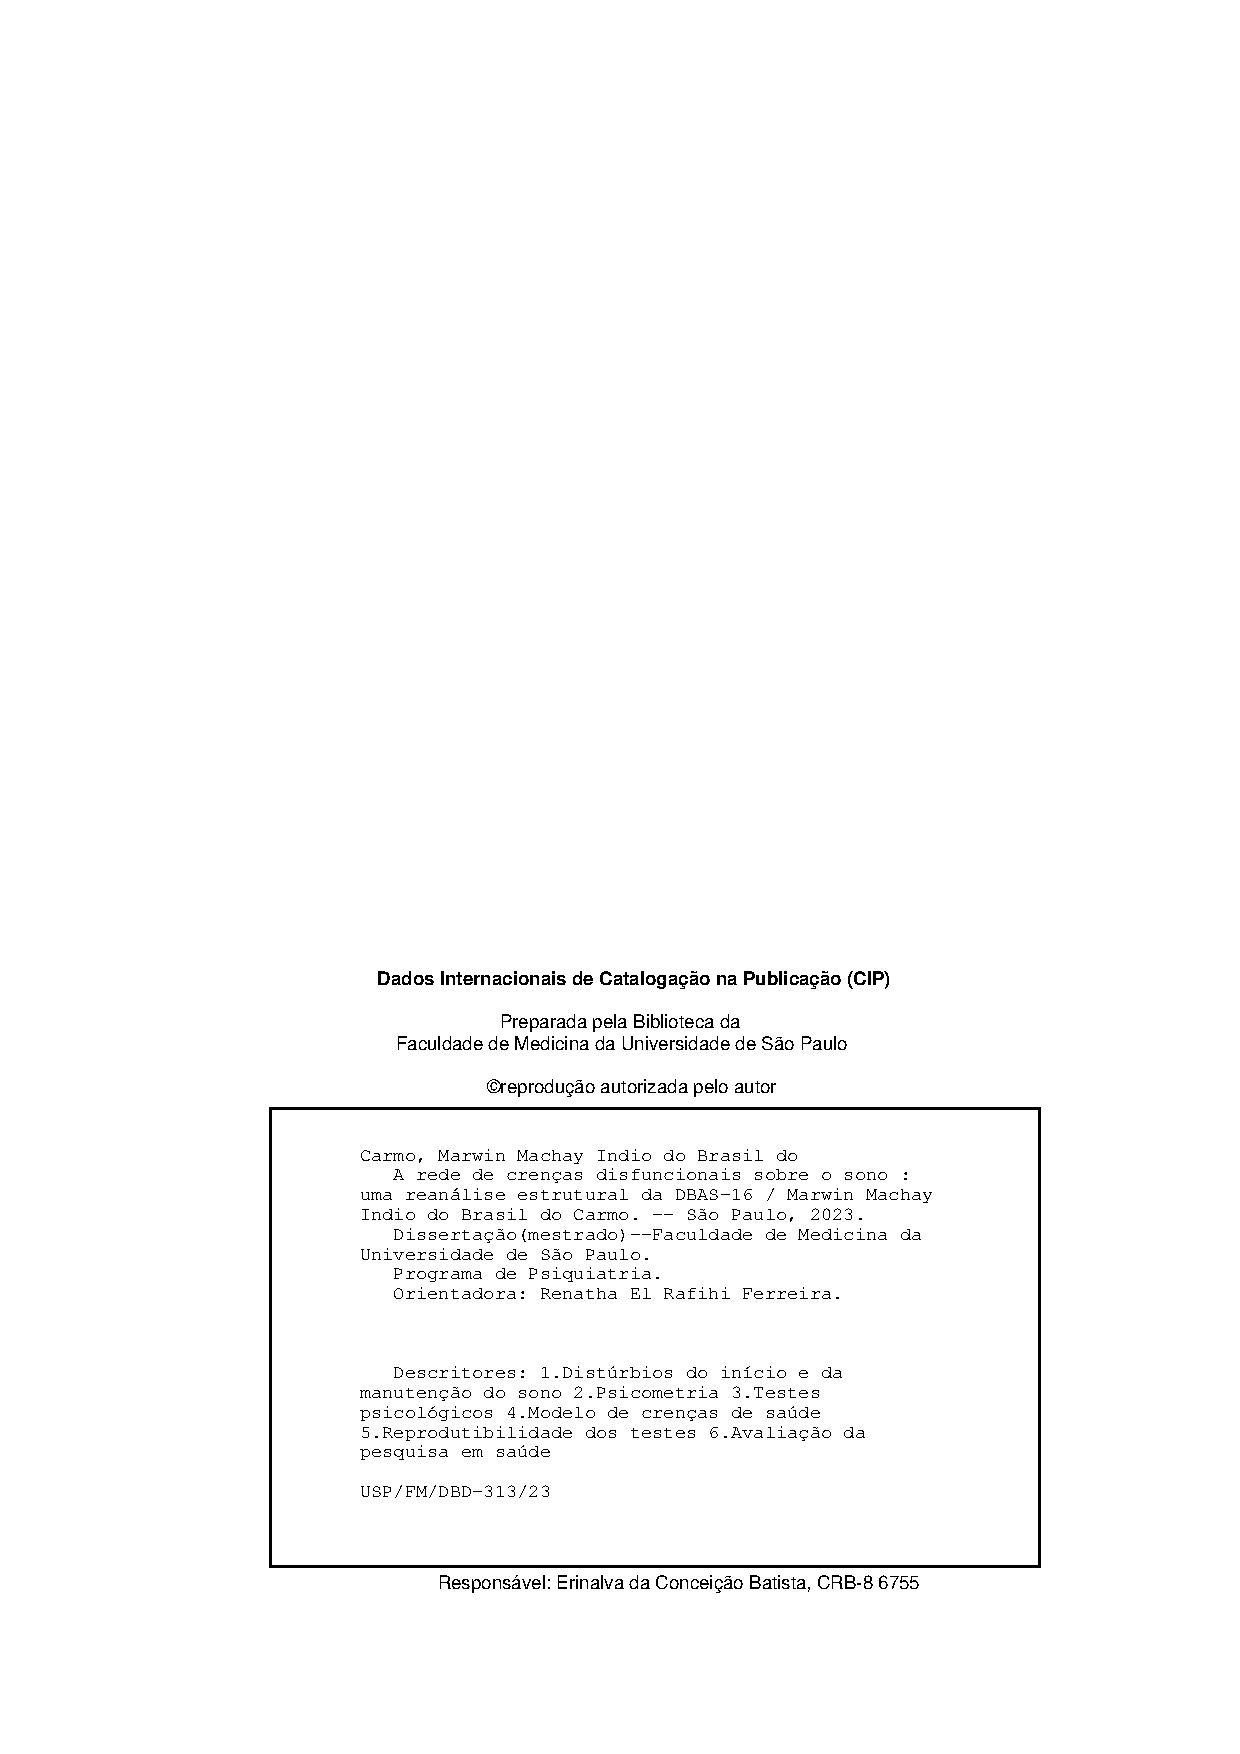
\includepdf[pages={1}]{ficha-catalog.pdf}
\end{fichacatalografica}


% \begin{fichacatalografica}
% 	\sffamily
% 	\vspace*{\fill}					% Posição vertical
% 	\begin{center}					% Minipage Centralizado
% 	\fbox{\begin{minipage}[c][8cm]{15cm}		% Largura
% 	\small
% 	\imprimirautor
% 
% 	\hspace{0.5cm} \imprimirtitulo  / \imprimirautor. --
% 	\imprimirlocal, \imprimirdata-
% 
% 	\hspace{0.5cm} \thelastpage p. : il. (algumas color.) ; 30 cm.\\
% 
% 	\hspace{0.5cm} \imprimirorientadorRotulo~\imprimirorientador\\
% 
% 	\hspace{0.5cm}
% 	\parbox[t]{\textwidth}{\imprimirtipotrabalho~--~\imprimirinstituicao,
% 	\imprimirdata.}\\
% 
% 	\hspace{0.5cm}
% 		1. Palavra-chave1.
% 		2. Palavra-chave2.
% 		2. Palavra-chave3.
% 		I. Orientador.
% 		II. Universidade xxx.
% 		III. Faculdade de xxx.
% 		IV. Título
% 	\end{minipage}}
% 	\end{center}
% \end{fichacatalografica}

% folha de aprovação 
%
%\begin{folhadeaprovacao}
%    \includepdf{folhadeaprovacao_final.pdf}
%\end{folhadeaprovacao}


% substituir pela folha assinada pela banca após defesa 
\begin{folhadeaprovacao}

  \begin{center}
    {\ABNTEXchapterfont\large\imprimirautor}

    \vspace*{\fill}\vspace*{\fill}
    \begin{center}
      \ABNTEXchapterfont\bfseries\Large\imprimirtitulo
    \end{center}
    \vspace*{\fill}
    
    \hspace{.45\textwidth}
    \begin{minipage}{.5\textwidth}
        \imprimirpreambulo
        \vspace*{1cm}
        Trabalho aprovado em:\\[2cm]
        \textbf{Banca Examinadora} \\
        \assinatura{\textbf{\imprimirorientador} \\ Universidade de São Paulo \\ Orientadora} 
        \assinatura{\textbf{Dra. Ila Marques Porto Linares} \\ Universidade Federal De São Paulo}
        \assinatura{\textbf{Dr. Altay Alves Lino de Souza} \\ Universidade Federal De São Paulo}
        %\assinatura{\textbf{Professor} \\ Convidado 3}
        %\assinatura{\textbf{Professor} \\ Convidado 4}
    \end{minipage}%
   \end{center}
  
\end{folhadeaprovacao}

%% dedicatória 
%\begin{dedicatoria}
%   \vspace*{\fill}
%   \centering
%   \noindent
%   \textit{Exemplo de dedicatória,\\\lipsum[10].} \vspace*{\fill}
%\end{dedicatoria}

%% agradecimentos 
%\begin{agradecimentos}
%\lipsum[30]
%
%\lipsum[30]
%
%\end{agradecimentos}

% epígrafe 
%\begin{epigrafe}
%    \vspace*{\fill}
%	\begin{flushright}
%		\textit{``Modelo de epígrafe, \\
%		modelo de epígrafe.''}
%	\end{flushright}
%\end{epigrafe}

% resumo 

\setlength{\absparsep}{18pt}
\begin{resumo}[Resumo]
  
  A insônia é um problema comum que afeta uma parcela significativa da população. Crenças e atitudes disfuncionais sobre o sono contribuem para o desenvolvimento e a manutenção da insônia. Este estudo desenvolveu uma versão em português brasileiro da escala Dysfunctional Beliefs and Attitudes about Sleep (DBAS-16) e realizou uma avaliação psicométrica abrangente usando técnicas de modelagem de variáveis latentes e redes psicométricas. Os participantes (N = 1.386) tinham entre 18 e 59 anos, com e sem queixas de insônia. Usando Análise Fatorial Confirmatória (AFC) com índices de ajuste dinâmico, a estrutura original do DBAS-16 foi replicada nesta amostra com qualidade de ajuste moderada. Houve também suporte para invariância longitudinal (14 dias) configural, métrica e escalar, mas não para invariância métrica entre grupos de bons e maus dormidores. A Unique Variable Analysis aplicada a metade dos dados da amostra (\emph{n} = 693) identificou três itens redundantes adequados para exclusão (1. \emph{Necessidade de 8 horas} de sono, 3. \emph{Consequências da insônia para a saúde} e 15. \emph{Medicação como solução}). Além disso, a Análise Exploratória de Grafos (EGA) identificou duas dimensões com excelente estabilidade estrutural, replicada quando a EGA foi aplicada à outra metade da amostra. Usando AFC, foi encontrado que o modelo obtido por EGA se ajustava significativamente melhor do que o modelo teórico proposto, endossando uma dimensionalidade alternativa da DBAS. Esses achados apoiam o uso do DBAS-16 com uma população de língua portuguesa brasileira. Além disso, após a exclusão de variáveis localmente dependentes, duas dimensões representaram melhor as crenças e atitudes disfuncionais sobre o sono.

  \textbf{Palavras-chave}: Distúrbios do Início e da Manutenção do Sono, Psicometria, Testes Psicológicos, Modelo de Crenças de Saúde, Reprodutibilidade dos Testes, Avaliação da Pesquisa em Saúde.
\end{resumo}

% abstract 
\begin{resumo}[Abstract]
  \begin{otherlanguage*}{english}
  
    Insomnia is a common problem that affects a significant portion of the population. Dysfunctional beliefs and attitudes about sleep contribute to developing and maintaining insomnia. This study developed a Brazilian-Portuguese version of the dysfunctional beliefs and attitudes about sleep scale (DBAS-16) and conducted a comprehensive psychometric evaluation using latent variable and psychometric network frameworks. Participants (N = 1,386) were between 18 and 59 years old, with and without insomnia complaints. Using Confirmatory Factor Analysis (CFA) with dynamic fit indices, the original DBAS-16 structure was replicated in this sample with moderate fit quality. There was also support for configural, metric, and scalar longitudinal invariance (14 days) but not for metric invariance across groups of good and bad sleepers. Unique Variable Analysis applied to half of the sample data (\emph{n} = 693) identified three redundant items suitable for exclusion (1. \emph{Need 8 hours of sleep}, 3. \emph{Consequences of insomnia on health}, and 15. \emph{Medication as a solution}). Additionally, Exploratory Graph Analysis (EGA) identified two dimensions with excellent structural stability, replicated when EGA was applied to the other half of the sample. Using CFA, it was found that the EGA model fit significantly better than the proposed theoretical model, endorsing an alternative DBAS dimensionality. These findings support the use of the DBAS-16 with a Brazilian-Portuguese-speaking population. Further, after excluding locally dependent variables, two dimensions better represent dysfunctional beliefs and attitudes about sleep.

    \vspace{\onelineskip}
 
    \noindent 
    \textbf{Keywords}: Sleep Initiation and Maintenance Disorders, Psychometrics, Psychological Tests, Health Belief Model, Reproducibility of Results, Health Research Evaluation.
  \end{otherlanguage*}
\end{resumo}

% lista de ilustrações 
\pdfbookmark[0]{\listfigurename}{lof}
\listoffigures*
\cleardoublepage

% lista de quadros 
% \pdfbookmark[0]{\listofquadrosname}{loq}
% \listofquadros*
% \cleardoublepage

% lista de tabelas 
\pdfbookmark[0]{\listtablename}{lot}
\listoftables*
\cleardoublepage

% lista de abreviaturas 
% \begin{siglas}
%   \item[MinT] \textit{Minimum Trace}
%   \item[MCRL] Modelo Clássico de Regressão Linear
%   \item[MQO] Mínimos Quadrados Ordinários
%   \item[MQP] Mínimos Quadrados Ponderados
%   \item[MQGF] Mínimos Quadrados Generalizados Factíveis
%   \item[ANN] \textit{Artificial Neural Network}
%   \item[SVR] \textit{Support Vector Regression}
%   \item[SFN] Sistema Financeiro Nacional
%   \item[Favar] \textit{Factor Augmented Vector Autoregression}
%   \item[Lasso] \textit{Least Absolute Shrinkage and Selection Operator}
% \end{siglas}

% lista de símbolos 
% \begin{simbolos}
%   \item[$ t $] Tempo dentro da amostra
%   \item[$ T $] Último tempo dentro da amostra, quantidade de observações numa série
%   \item[$ h $] Horizonte de previsão, tempo fora da amostra
%   \item[$ \Omega $] Conjunto de dados dentro da amostra
%   \item[$ y $] Série temporal dentro da amostra
%   \item[$ \hat{y} $] Série temporal estimada
%   \item[$ \tilde{y} $] Série temporal reconciliada
%   \item[$ n $] Número de séries na hierarquia
%   \item[$ m $] Número de séries no menor nível da hierarquia
%   \item[$ k $] Número de níveis na hierarquia
%   \item[$ \mathbfit{S} $] Matriz de soma
%   \item[$ \mathbfit{G} $] Matriz de reconciliação
%   \item[$\{...\}$] Conjunto
%   \item[$|\{...\}|$] Cardinalidade de um conjunto
% \end{simbolos}

% sumário 
\pdfbookmark[0]{\contentsname}{toc}
\tableofcontents*

% elementos textuais 
\textual
\pagestyle{simple}

\ifdefined\Shaded\renewenvironment{Shaded}{\begin{tcolorbox}[interior hidden, borderline west={3pt}{0pt}{shadecolor}, sharp corners, boxrule=0pt, breakable, enhanced, frame hidden]}{\end{tcolorbox}}\fi

\hypertarget{introduction}{%
\section{INTRODUCTION}\label{introduction}}

Insomnia is a disorder characterized by dissatisfaction with sleep
duration or quality \autocite{americanpsychiatricassociation2013}.
Several cognitive and behavioral models of insomnia emphasize the role
of sleep-related thoughts in perpetuating the disorder
\autocite{espie2006,harvey2002,lundh2005,morin1993,ong2012,perlis1997}.
The frequently referenced model of A. G. Harvey \autocite*{harvey2002}
proposes that negative thoughts and behaviors about sleep can trigger
arousal and distress, leading to distorted perceptions of sleep and
increased worry. These beliefs may also exacerbate cognitive activity
and prevent sleep self-correction. The Microanalytic model
\autocite{morin1993} is also based on similar beliefs and is popular
among experts studying insomnia processes \autocite{marques2015}.

Current evidence suggests that beliefs and attitudes about sleep play a
role in perpetuating insomnia
\autocite{akram2020,chow2018,harvey2017,lancee2019}, although some
studies do not support this association \autocite{norell-clarke2021}.
The Microanalytic model \autocite{morin1993} proposes that insomnia
maintenance involves a cyclic process of arousal, dysfunctional
cognitions, maladaptive habits, and consequences. Arousal refers to
excessive emotional, cognitive, or physiological activity, which can
create core beliefs that guide information processing
\autocite{marques2015}. Consequences may include unrealistic
expectations, rigid beliefs about sleep requirements, and increased
worry about the causes and consequences of sleep disturbances.
Subsequent unhealthy sleep practices may include daytime napping,
excessive time in bed, or indiscriminate use of sleep medication. Real
or perceived consequences are linked to diminished performance during
the day \autocite{sullivan2022}.

\hypertarget{constructs-and-their-relations}{%
\subsection{Constructs and Their
Relations}\label{constructs-and-their-relations}}

Individuals with higher insomnia symptoms are typically strong endorsers
of dysfunctional beliefs about sleep
\autocite{carney2006,cronlein2014,eidelman2016}. Cognitive-behavioral
treatments target modifying such unhelpful beliefs and habits about
sleep, leading to objective and subjective sleep quality improvements
\autocite{harvey2014,montserratsanchez-ortuno2010,belanger2006}. CBT-I
has been shown to significantly improve beliefs and attitudes about
sleep compared to controls, although the evidence quality is low
\autocite{edingerjackd.2021}.

Insomnia severity is a risk factor for anxiety \autocite{neckelmann2007}
and depression \autocite{blanken2020,li2016}, but some suggest the
relationship may be reversed \autocite{chen2017,jansson-frojmark2008b}.
A link between anxiety, depression, and dysfunctional beliefs about
sleep is also expected. Beck's \autocite*{beck1979cognitive} cognitive
model for depression emphasizes inaccurate beliefs and maladaptive
information processing. Unpleasant memories from negative experiences
can cause anxiety \autocite{brewin1996theoretical}. Thus, unrealistic
attributions and expectations about sleep can lead to anxiety-provoking
thoughts. There is also evidence that dysfunctional beliefs about sleep
are an indirect pathway between insomnia and depression
\autocite{sadler2013}.

\hypertarget{measurement-of-dysfunctional-beliefs-and-attitudes-about-sleep}{%
\subsection{Measurement of dysfunctional beliefs and attitudes about
sleep}\label{measurement-of-dysfunctional-beliefs-and-attitudes-about-sleep}}

The Dysfunctional Beliefs and Attitudes About Sleep Scale
\autocite[DBAS,][]{morin1993insomnia} is one of the earliest tools to
evaluate sleep-related beliefs and attitudes. It is often used in
research studies that examine sleep-related thoughts, particularly the
16-question version \autocite{thakral2020}. Originally a 30-item
self-report measure rated on a 100-mm scale of agreement/disagreement,
it was shortened to 16 items and rated on an 11-point scale ranging from
0 (strongly disagree) to 10 (strongly agree) \autocite{morin2007a}. The
16 items were selected based on response distribution, item-total
correlations, and exploratory oblique factor analysis.

A Confirmatory Factor Analysis was used to fit a 4-factor structure to
the 16 items, with factors labeled (a) consequences of insomnia, (b)
worry about sleep, (c) sleep expectations, (d) medication, and a fifth
second-order general factor. \textcite{morin2007a} have reported
acceptable fit indices for the DBAS-16 but highlighted that items 10
(``sleep is unpredictable'') and 13 (``insomnia resulting from chemical
imbalance'') with very low item-total correlations and factor loadings
were kept because of their clinical relevance. Researchers have
translated and validated the DBAS-16 across various cultures
\autocites[e.g.,][]{boysan2010,dhyani2013,lang2017}, reporting good
validity evidence overall.

Before the development of the DBAS-16, alternative versions of the scale
were proposed. \textcite{espie2000} created a 10-item version based on
the item's statistically significant score change after
cognitive-behavioral therapy for insomnia. However, Edinger and
Wohlgemuth's \autocite*{edinger2001a} replication study did not fully
reproduce the 3-factor structure of this version. Moreover,
\textcite{chungka-fai2016} found that the DBAS-16 outperformed 30- and
10-item versions in reproducibility, internal consistency, concurrent
validity, and sensitivity to change.

Recently, \textcite{castillo2023} analyzed the DBAS-16 using Item
Response Theory (IRT) with university students. They discovered that the
``medication'' and ``expectations'' factors had the lowest test
information, while the ``worry/helplessness'' and ``consequences''
subscales were highly informative in measuring the latent construct.
Furthermore, the authors shortened the test by removing items 10, 13,
and 16 to improve model fit.

\textcite{clemente2023} proposed a 16-item version (DBAS-SF-16) of
Morin's DBAS-30 after refining the scale items through sequential
psychometric analysis. Exploratory factor analysis revealed two factors:
``Consequences and Helplessness'' and ``Medication and Hopelessness.''
Four items from Morin's DBAS-16 did not meet the criteria for inclusion
in DBAS-SF-16.

\hypertarget{the-present-study}{%
\subsection{The Present Study}\label{the-present-study}}

In the study and treatment of insomnia, it is important to consider
dysfunctional beliefs about sleep. The Dysfunctional Beliefs About Sleep
questionnaire is essential to assess this. Examining the psychometric
properties of any measure used to evaluate unobservable constructs is
crucial to ensure precision \autocite{mcneish2022a}. There have been
discrepancies among studies regarding the DBAS items and factors'
accuracy in representing the underlying construct, indicating a need for
additional psychometric research on this measurement tool.

The present study has two primary aims: 1) to create a
Brazilian-Portuguese adaptation of the Dysfunctional Beliefs and
Attitudes about Sleep Scale (DBAS-16). Using latent variable modeling,
we will analyze its factorial structure, reliability, and construct
validity. 2) To conduct an exploratory analysis using a psychometric
network perspective. This approach models psychopathology as a network
of causal interactions among symptoms rather than originating from a
root cause, such as latent variable models, and has gained popularity in
psychiatry and psychology
\autocite{borsboom2008,borsboom2013,bringmann2022}.

\hypertarget{methods}{%
\section{METHODS}\label{methods}}

\hypertarget{study-design-and-setting}{%
\subsection{Study design and setting}\label{study-design-and-setting}}

The current study is linked to a randomized controlled trial (RCT) of
behavioral treatment for insomnia (Clinical trial: NCT04866914). The
study was approved by the research ethics committee of the General
Hospital of the University of São Paulo, School of Medicine (HC-FMUSP),
São Paulo, Brazil (CAAE: 46284821.1.0000.0068). All participants signed
a consent form prior to their inclusion. Participants then completed an
online survey using REDCap electronic data capture tools
\autocite{harris2019redcap}, including the Brazilian-Portuguese version
of DBAS-16 and other auxiliary instruments. In order to test temporal
stability, the same participants were emailed and asked to complete the
same measures again 14 days later. This study was not preregistered. The
R code, dataset, and RMarkdown file containing the manuscript text used
in this paper can be accessed at
\href{https://osf.io/qcbwn/}{osf.io/qcbwn}.

\hypertarget{sample-size}{%
\subsection{Sample size}\label{sample-size}}

To estimate an adequate sample size, we used MacCallum et al.'s
\autocite*{maccallum1996} root-mean-square error of approximation
(RMSEA) tests of close and not-close fit for the confirmatory factor
analysis (CFA). We performed these tests in R 4.3.0 \autocite{R-base}
using \emph{semTools} version 0.5.6 \autocite{semtools}. Morin
\autocite*{morin2007a} previously reported an RMSEA of 0.059 for DBAS-16
in a CFA. Using this value as a starting point, we calculated the sample
sizes needed to reject the test of not-close fit with an RMSEA value
greater than 0.08 and the test of close fit with an RMSEA value less
than 0.05, both with a power of 0.80 and a significance level of 0.05.
Our calculations indicated that a minimum of 216 subjects were necessary
to reject the not-close fit test, and 924 participants were required to
reject the close fit test. Based on this information, our target sample
size was set at a minimum of 924 participants.

\hypertarget{participants}{%
\subsection{Participants}\label{participants}}

Participants with and without insomnia were recruited from March 2021 to
July 2022 through social media. The first group consisted of individuals
already enrolled in behavioral treatment for insomnia. To include
participants without insomnia, we requested volunteers who believed they
had no sleeping issues. Interested individuals accessed the REDCap
database platform and responded to an initial screening. The inclusion
criteria were age between 18 and 59 years and had no reported
difficulties reading or writing in Portuguese.

Bad sleepers were categorized based on their complaints of insomnia.
This includes experiencing difficulty falling asleep or staying asleep,
as per the Diagnostic and Statistical Manual of Mental Disorders
\autocite{americanpsychiatricassociation2013} criteria. Additionally,
participants' total score on the Insomnia Severity Index should not
exceed 7 points \autocite{bastien2001}. The participants were classified
as good sleepers if none of these criteria was met.

After removing those who did not complete a single item of DBAS-16 on
the first administration, the final sample consisted of 1389
participants, of which 80.78\% were female, and 73.51\% reported
insomnia symptoms. The mean age was 38.39 years (SD = 9.79, range:
18--59). Among those who reported race, there were 71.78\% Whites,
23.83\% Blacks, and 3.46\% Asians. Most had a university degree
(77.75\%) and were active workers (76.96\%).

\hypertarget{material}{%
\subsection{Material}\label{material}}

\hypertarget{dysfunctional-beliefs-and-attitudes-about-sleep-scale-dbas-16}{%
\subsubsection{Dysfunctional Beliefs and Attitudes About Sleep Scale
(DBAS-16)}\label{dysfunctional-beliefs-and-attitudes-about-sleep-scale-dbas-16}}

To develop a Brazilian-Portuguese version of the DBAS-16, we mainly
based our methods on Beaton's \autocite*{beaton2000} recommendations
with additions from \textcite{borsaAdaptacaoValidacaoInstrumentos2012}.
The original English version was translated by three independent
translators, two familiar with the instrument constructs and one an
English teacher with no medical background. A committee of two clinical
psychologists experts in insomnia synthesized the translated versions
documenting their decisions in a form. Then, two native speakers of the
source language back-translated the synthesized version to English for
review by the first author of the original questionnaire. Next, we
conducted a cognitive debriefing with 15 participants from different
regions and educational levels to test the pre-final version. Of the
participants, 12 were female, and the mean age was 43 years (range:
19--57). Overall, the participants understood the test items and
instructions well, and only one term required alteration for better
readability in the target language. The final translation is available
as supplementary material, and all intermediate versions are available
at \href{https://osf.io/av45j/}{osf.io/av45j}.

\hypertarget{additional-measures}{%
\subsubsection{Additional measures}\label{additional-measures}}

\begin{enumerate}
\def\labelenumi{\arabic{enumi}.}
\item
  \emph{Insomnia Severity Index}
  \autocites[ISI,][]{bastien2001,morin2011a} is a seven-item
  questionnaire that assesses the severity of insomnia and its impact on
  a person's life. The scale ranges from 0 (no problems) to 4 (very
  severe problem) and categorizes respondents as having no insomnia
  (0--7), mild insomnia (8--14), moderate insomnia (15--21), or severe
  insomnia (22--28). For our study, we used the Brazilian-Portuguese
  version \autocite{castro}. A Confirmatory Factor Analysis (CFA) of the
  single-factor model produced an acceptable fit: \(\chi^2\) (14) =
  342.35, \emph{p} \textless{} .001 RMSEA = .128 90\% CI {[}.117,
  .140{]}, CFI = .996, SRMR = .047, and good internal consistency
  reliability: \(\omega_h\) = .942 {[}.937, .947{]}.
\item
  \emph{The Hospital Anxiety and Depression Scale}
  \autocite[HADS,][]{zigmond1983hospital} assesses psychological
  distress in non-psychiatric patients through two factors: Anxiety and
  Depression. Each factor has seven items that only measure emotions,
  not somatic symptoms. The score ranges from 0 to 21 for each factor.
  Scores of 0 to 8 indicate no anxiety/depression, while nine and above
  indicate their presence. The Brazilian-Portuguese version created by
  \textcite{botega1995transtornos} was used. A two-factor model produced
  excellent CFA fit indices: \(\chi^2\) (76) = 572.01, RMSEA = .068 90\%
  CI {[}.063, .073{]}, CFI = .993, SRMR = .047, and good internal
  consistency reliability for both factors: \(\omega_{h-depression}\) =
  .876 {[}.866, .886{]}, \(\omega_{h-anxiety}\) = .884 {[}.874, .892{]}.
\end{enumerate}

\hypertarget{data-analysis}{%
\subsection{Data analysis}\label{data-analysis}}

\hypertarget{data-screening-and-item-evaluation}{%
\subsubsection{Data screening and item
evaluation}\label{data-screening-and-item-evaluation}}

First, we examined response frequency and item statistics to assess item
variation, distribution, and data entry. We also investigated inter-item
correlations and searched for unusual response patterns by identifying
multivariate outliers using Mahalanobis distance. Additionally, we used
the generalized Cook's distance (gCD) with the R package
\emph{faoutlier} version 0.7.6 \autocite{faoutlier} to identify any
points of influence.

\hypertarget{assessing-the-factor-structure}{%
\subsubsection{Assessing the factor
structure}\label{assessing-the-factor-structure}}

We fitted the original model of the DBAS-16 \autocite{morin2007a} to our
full sample using Confirmatory Factor Analyses (CFA) as a first test for
structural validity. This model is a four-factor structure and a
higher-order general factor. But because the DBAS-16 is often modeled
with disregard for the higher-order factor
\autocite{lang2017,castillo2023,boysan2010,clemente2023}, we also tested
a four-factor model allowing factors to covary and compared the fit of
both. We used normal theory maximum likelihood (ML) to estimate the
structural model parameters \autocite{rhemtulla2012}. To account for the
severe non-normality in our data, we applied maximum likelihood
estimation with robust standard errors and a mean and variance-adjusted
test statistic (MLMV) \autocite{maydeu-olivares2017}. Our model fit
evaluation relied on fit statistics including, chi-squared (\(\chi^2\)),
Comparative Fit Index (CFI), Root Mean Square Error of Approximation
(RMSEA), and Standardized Root Mean Squared Residual (SRMR). Obtaining
confidence intervals (CI) for robust RMSEA and CFI involved computing
the second-order corrected RMSEA CI based on the MLMV test statistic
\autocite{savalei2018}. All the CFA analyses were conducted with the R
packages \emph{lavaan} version 0.6.12 \autocite{R-lavaan} and
\emph{semTools} version 0.5-6 \autocite{R-semTools}.

Traditionally, CFA studies use cutoff values of SRMR \(\le\) .08, RMSEA
\(\le\) .06, and CFI, TLI, and RNI \(\ge\) .96 to evaluate model
misspecification \autocite{hu1999}. These values have limitations
because they were derived from particular conditions, making
generalizations to other models limited and unwarranted
\autocite{marsh2004}. Therefore, another advantage of using a ML
estimation method is using dynamic fit index (DFI) cutoffs
\autocite{mcneish2021}. In essence, DFI provides cutoff values that
would have been derived had our model been used in simulations similar
to the one conducted by Hu and Bentler \autocite*{hu1999}. DFI is
calculated based on the number of factors in the model and assesses
misspecification severity at sequential levels. We used the Dynamic
Model Fit R Shiny application version 1.1.0 \autocite{wolf2020} to
obtain DFI for our models.

\hypertarget{measurement-invariance}{%
\subsubsection{Measurement invariance}\label{measurement-invariance}}

We examined whether our scale's psychometric properties were equal
across groups with and without insomnia symptoms and across time points,
comparing baseline test scores to a second administration taken 14 days
later. To do this, we tested invariance by restricting the measurement
properties across groups/time in increasing levels of stringency. We
tested in a sequence of factor structure (configural invariance), factor
loadings (metric invariance), items' intercepts (scalar invariance), and
items' residual variances (strict invariance) \autocite{flake2021}. If a
level of non-invariance was detected, no further tests were conducted.
The criteria used to evaluate model fit were the chi-squared difference
test for goodness of fit and alternative fit indices like \(\Delta\)CFI,
\(\Delta\)RMSEA, and \(\Delta\)SRMR \autocite{putnick2016}. While there
are suggested cutoffs for alternative fit indices that indicate a lack
of invariance \autocites[e.g.,][]{cheung2002,meade2008,chen2007}, these
are still limited because researchers can only test a narrow set of
conditions \autocite{putnick2016}. Thus, we used a global approach that
tested differences in fit between the restricted and less-constrained
models in each stage, also looking at comparative fit measures of Akaike
information criterion (AIC) and the Bayesian information criterion (BIC)
\autocite{mackinnon2022}. We gave greater weight to BIC results because
it performs better in different simulation scenarios \autocite{lin2017}.

\hypertarget{reliability-and-validity}{%
\subsubsection{Reliability and
validity}\label{reliability-and-validity}}

We used McDonald's omega hierarchical (\(\omega_h\)) to estimate
internal consistency. This measure has advantages over Cronbach's
\(\alpha\), as it does not assume tau equivalence (i.e., loadings are
not assumed equal) or a perfect fit in CFA \autocite{kelley2016}. We
calculated the point estimate and the bias-corrected and accelerated
bootstrap confidence interval (1000 bootstrap samples) for the internal
consistency indices using the R package \emph{MBESS} version 4.9.2
\autocite{MBESS}. We followed the traditional guideline of internal
consistency indices \(\ge\) .70 to evaluate reliability as acceptable
\autocite{kline1986}.

To assess convergent validity, we estimated a structural equation model
where the DBAS-16 factors, insomnia severity, and the HADS subscales of
depression and anxiety were allowed to correlate. We expect these
associations to be positive and strong. These associations were also
explored in a network model, where variables are represented as nodes,
and their connections by weighted edges, representing their conditional
associations \autocite{borsboom2021}. We used \emph{bootnet} version 1.5
\autocite{R-bootnet} to estimate the network and \emph{qgraph} version
1.9.4 \autocite{R-qgraph} to create the plot.

\hypertarget{network-psychometrics}{%
\subsubsection{Network psychometrics}\label{network-psychometrics}}

We divided our sample into two equal parts and conducted this phase in
stages of derivation and confirmation. In the derivation step, we aimed
to obtain an optimal network structure using a redundancy analysis,
dimension analysis, and internal structure analysis based on the methods
outlined by \textcite{christensen2020b} to test validity from the
network perspective. We were also inspired by
\textcite{flores-kanter2021} analysis of the Positive and Negative
Affective Schedule (PNAS). In the confirmation phase, we tested if our
obtained solution was replicated and tested its plausibility against the
theoretical model using CFA. We also tested measurement invariance
across good and bad sleepers within the Exploratory Graph Analysis (EGA)
framework. To perform these analyses, we used the \emph{EGAnet}
\autocite{EGAnet} package for R and visualized the associated results
using the \emph{GGally} version 2.1.2 \autocite{R-GGally},
\emph{ggplot2} version 3.4.2 \autocite{R-ggplot2}, and \emph{qgraph}
version 1.9.4 \autocite{R-qgraph} packages in R.

When modeling psychological data, redundant items can lead to unintended
effects, make it difficult to interpret centrality measures in network
models, and violate the principle of local independence in latent
variable models \autocite{christensen2023}. Unique Variable Analysis
\autocite[UVA,][]{christensen2023} can identify redundant items using
network modeling and a graph theory measure called weighted topological
overlap (wTO). UVA identifies locally dependent pairs of variables and
uses the false discovery rate (FDR) to assess the expected count of
false positives. This algorithm first computes the association structure
of the observed data, then uses a threshold or significance test to
determine redundancy between pairs of variables. The redundant variables
can be removed, leaving only one non-redundant indicator, or aggregated
as latent variables. Redundant pair of items were identified as those in
which the weighted topological overlap exceeded the cutoff value of .25.
Following Christensen's (personal communication, June 26, 2023)
recommendations, when dealing with three or more redundant items, we
kept the one with the highest average wTO to all other redundant items
in the group. For two redundant items, we kept the one with the lowest
maximum wTO to all other items. When inconclusive, we also considered
factors such as item-test correlation, variance, and representation of
the attribute \autocite{christensen2020a}.

To estimate the number of dimensions, we used Exploratory Graph Analysis
\autocites[EGA,][]{golino2017,golino2020}, a recently developed method
of dimensionality assessment from network psychometrics. This method
employs undirected network models to determine the number of dimensions
in multivariate data. Firstly, the EGA algorithm estimates the network
using either the Graphical Least Absolute Shrinkage and Selection
Operator \autocites[GLASSO,][]{R-glasso,friedman2008} or the
Triangulated Maximally Filtered Graph \autocite[TMFG,][]{massara2016}.
Then, it applies a community detection algorithm to identify the number
and content of communities in the network. These communities are
statistically equivalent to factors of latent variable models
\autocite{golino2017}. As recommended by \textcite{golino2020}, we used
both GLASSO and TMFG methods to estimate the psychometric networks. One
advantage of the TMFG method is that it is appropriate for skewed
distributions, which is the case with our data
\autocite{christensen2018,christensen2023a}. We employed the Walktrap
algorithm for community detection in both methods. This algorithm is
popular in the psychometric network literature and effectively retrieves
the correct number of dimensions \autocite{golino2020,christensen2023a}.
To select the best solution in case of differences, we employed the
\emph{total entropy fit index with Von Neumman entropy}
\autocite[TEFI.vn,][]{golino2021a}. Structures with lower entropy better
reflect the underlying latent factors \autocite{golino2021a}. Spearman's
rho correlation was used to compute the correlation matrix for the
network estimation methods. EGA has shown more promising results in
estimating the number of dimensions than traditional factor analytic
methods, such as Parallel Analysis, especially in structures with four
or more factors \autocite{golino2020}.

To determine if our data was unidimensional, we used the Leading
Eigenvalue algorithm \autocite{newman2006}. This algorithm was applied
to the correlation matrix, and if a single dimension was identified,
this indicated unidimensionality. Conversely, the standard EGA procedure
was followed if multiple dimensions were identified. Based on
simulations conducted by \textcite{christensen2023a}, this algorithm
proved more effective in achieving a balanced recovery of one and two
factors.

We also investigated configural and metric invariance across groups of
good and bad sleepers using EGA. Configural invariance in EGA indicates
that the same nodes are partitioned into the same communities for all
groups, and metric invariance employs permutation testing to verify
whether network loadings are equivalent across groups
\autocite{jamison2022}. Network loadings represent the unique
contribution of each node to the emergence of a dimension in a network
\autocite{christensen2021}.

Computing internal consistency measures from a network perspective is
not feasible due to the common covariance between items being removed in
network models \autocite{christensen2020b}. However, to address this
issue, \textcite{christensen2020b} suggest examining ``the extent to
which items in a dimension are homogeneous and interrelated given the
multidimensional structure of the questionnaire'' (p.~8), which they
refer to as \emph{structural consistency}. This measure was estimated
using Bootstrap Exploratory Graph Analysis
\autocite[bootEGA,][]{christensen2021a}. BootEGA generates a sampling
distribution of EGA results from replicate data. It informs how often
dimensions are exactly recovered (structural consistency) and how often
each item is allocated in its respective empirical dimension (item
stability). Structural consistency and item stability are between 0 and
1, and values above 0.75 are acceptable for both. The bootstrap results
are summarized in median, standard error, 95\% confidence intervals, and
frequency of which a certain number of dimensions replicates.
Additionally, bootEGA provides a measure of the typical network
structure of the sampling distribution. A single network is estimated by
computing the median value of each edge across the replicate networks
and applying the community detection algorithm.

\hypertarget{results}{%
\section{RESULTS}\label{results}}

\hypertarget{data-screening}{%
\subsection{Data screening}\label{data-screening}}

We used Mahalanobis distance (MD) to scan for multivariate outliers and
found 27 respondents with D\textsuperscript{2} values with probability
values \textless.001 (df = 16). After examining the item statistics, we
determined that all observations fell within the possible range of
scores, eliminating the possibility of outliers resulting from data
collection or entry errors. Therefore, no observations were excluded.

In factor analysis, outliers may not influence model fit or parameter
estimates \autocite{pek2011}. To identify leverage points in our sample,
we used the generalized Cook's distance (gCD) statistic, which measures
the amount of change in a group of parameter estimates when an
observation is excluded \autocite{pek2011}. We calculated a gCD value
for each observation in our sample and identified five highly
influential observations through a box-plot of gCD values
\autocite{flora2012}. These observations were excluded from the sample
to ensure the accuracy of our analysis.

\hypertarget{confirmatory-factor-analysis}{%
\subsection{Confirmatory Factor
Analysis}\label{confirmatory-factor-analysis}}

After comparing the fit of a higher-order structure with a four-factor
structure, we determined that the latter was a better fit for our data:
\(\Delta\chi^2\)(2) = 269.1, \emph{p} \textless{} .001, \(\Delta\)AIC =
-296.86, \(\Delta\)BIC = -286.4. We interpreted the four-factor
structure, despite some fit problems indicated by traditional cutoffs:
\(\chi^2\) (98, N = 1385) = 974.41, RMSEA = .094 90\% CI {[}.089,
.100{]}, CFI = .891, SRMR = .074. The model fit indices were slightly
worse than a Level-3 misspecification by DFI standaweights::rds (SRMR =
.051, RMSEA = .10, CFI = .922), indicating inconsistency even with large
misspecification, representing an omission of standardized
cross-loadings with magnitudes of .456, .443, and .464. Further
examination of the modification indices revealed that the model could be
improved by freeing correlations between residual variances of items 3
and 4 and between items 6 and 15. After making these changes, the model
fit indices improved and were more consistent with a Level-3
misspecification (SRMR = .051, RMSEA = .094, CFI = .936): \(\chi^2\)
(96, N = 1385) = 686.176, RMSEA = .077 90\% CI {[}.072, .083{]}, CFI =
.928, SRMR = .060.

\hypertarget{measurement-invariance-1}{%
\subsection{Measurement Invariance}\label{measurement-invariance-1}}

\begin{table}

\caption{Model fit differences for CFA measurement invariance tests.}
\centering
\begin{tabular}[t]{lrrlllrr}
\toprule
Model & $\Delta\chi^2$ & $\Delta$df & p-value & $\Delta$RMSEA & $\Delta$CFI & $\Delta$AIC & $\Delta$BIC\\
\midrule
\addlinespace[0.3em]
\multicolumn{8}{l}{\textbf{Longitudinal invariance}}\\
\hspace{1em}Configural & 1430.40 & 416 & <.001 & .0607 & .9364 & 164747 & 165474\\
\hspace{1em}Metric & 7.81 & 12 & .80 & .0007 & .0004 & 1 & 62\\
\hspace{1em}Scalar & 39.76 & 12 & <.001 & -.0005 & .0029 & -65 & -5\\
\hspace{1em}Strict & 91.84 & 16 & <.001 & -.0024 & .0081 & -208 & -127\\
\addlinespace[0.3em]
\multicolumn{8}{l}{\textbf{Group invariance}}\\
\hspace{1em}Configural & 496.26 & 164 & <.001 & .0643 & .9211 & 96100 & 96654\\
\hspace{1em}Metric & 57.43 & 11 & <.001 & -.0042 & .0168 & -91 & -34\\
\bottomrule
\multicolumn{8}{l}{\rule{0pt}{1em}\textit{Note. } Differences to each preceding constraint level.}\\
\end{tabular}
\end{table}

To analyze measurement invariance across insomnia severity status (good
and bad sleepers), we first tested the configural invariance model to
attest to the similarity of groups regarding the number of latent
constructs and the items loaded onto them. We found that the fit of this
model was acceptable, supporting configural invariance: \(\chi^2\) (164,
N = 1385) = 496.260, RMSEA = .064 90\% CI {[}.058, .071{]}, CFI = .921,
SRMR = .047. We proceeded then to test metric invariance (i.e., factor
loadings constrained to be equal across groups) but did not find any
evidence to support it. This is due to the significant difference in
chi-square between the configural and metric invariant models and the
AIC and BIC indices favoring the less restricted model (see
\textcite{fit-differences}). Since metric invariance was not achieved,
we did not test for stricter invariant models. These results show that
the indicators do not have the same relationship to the latent variables
in both groups.

Longitudinal measurement invariance of the DBAS-16 was tested similarly.
The configural invariant model showed adequate fit, allowing us to
continue with further testing. The metric invariant model showed no
significant differences in scaled chi-squared difference test,
indicating metric invariance across time. We then moved on to the scalar
invariance model, which assessed the equality of item responses
constraining the intercepts. There was a slight worsening in comparative
fit measures (\(\Delta\)CFI = .003, \(\Delta\)RMSEA = -.00049); however,
the change was considered negligible \autocite{chen2007,meade2008}. The
change in BIC was lower than 6, a value deemed evidence of model
difference \autocite{raftery1995}. Despite a significant increase in
chi-square, we believe that scalar non-invariance is minimal, if not
ignorable. However, we chose not to proceed with further testing to be
cautious.

\hypertarget{reliability-and-validity-1}{%
\subsection{Reliability and Validity}\label{reliability-and-validity-1}}

\hypertarget{internal-consistency}{%
\subsubsection{Internal consistency}\label{internal-consistency}}

The internal consistencies of each of the four dimensions were good,
with omega values ranging from .60 to .88. The DBAS-16 total score had
an \(\omega_h\) of .890 {[}.876, .902{]}, indicating good internal
consistency. It is important to note that the scale is not
unidimensional, and it is inappropriate to interpret it as such.
However, many studies interpret the total sum score to examine the level
of dysfunctional beliefs and behaviors about sleep, so we report the
internal consistency of the full scale. See
(\textcite{internal-consistency}) for full results of internal
consistency coefficients.

\begin{table}[!h]

\caption{Latent correlations and internal consistency levels.}
\centering
\begin{tabular}[t]{lllllc}
\toprule
Variable & 1 & 2 & 3 & 4 & $\omega_h$\\
\midrule
1. Consequences & 1.000 &  &  &  & .827 [.811, .843]\\
2. Worry & .693 & 1.000 &  &  & .882 [.871, .893]\\
3. Expectations & .569 & .101 & 1.000 &  & .600 [.557, .644]\\
4. Medication & .704 & .994 & .126 & 1.000 & .752 [.730, .771]\\
5. ISI & .508 & .937 & -.079 & .861 & .942 [.937, .947]\\
\addlinespace
6. Depression & .433 & .682 & .051 & .662 & .876 [.866, .886]\\
7. Anxiety & .421 & .719 & .020 & .676 & .884 [.874, .892]\\
\bottomrule
\end{tabular}
\end{table}

\hypertarget{convergent-validity}{%
\subsubsection{Convergent validity}\label{convergent-validity}}

DBAS-16 factors showed significant associations with depression,
anxiety, and insomnia severity with moderate to strong strength (except
``expectation'' scores), as shown in
(\textbf{?@tbl-internal-consistency}). The network in Figure
Figure~\ref{fig-network-conv} represents a joint partial correlation
structure of the DBAS-16 factors and these psychological variables. Each
weighted edge on this network is a conditional pairwise correlation
between two nodes controlling for all the other variables. The absence
of edges between nodes reflects weak partial correlations reduced to
zero due to the penalization for model complexity. Notably, there were
negligible relationships between depression and anxiety and any of the
four DBAS-16 factors after accounting for insomnia severity and either
of the two variables. The relations with insomnia severity were also
low, except for the Worry factor, which had the highest centrality
measures (see Figure~\ref{fig-network-conv}). The network also showed a
negative correlation between Expectations and insomnia severity.

\begin{figure}

{\centering 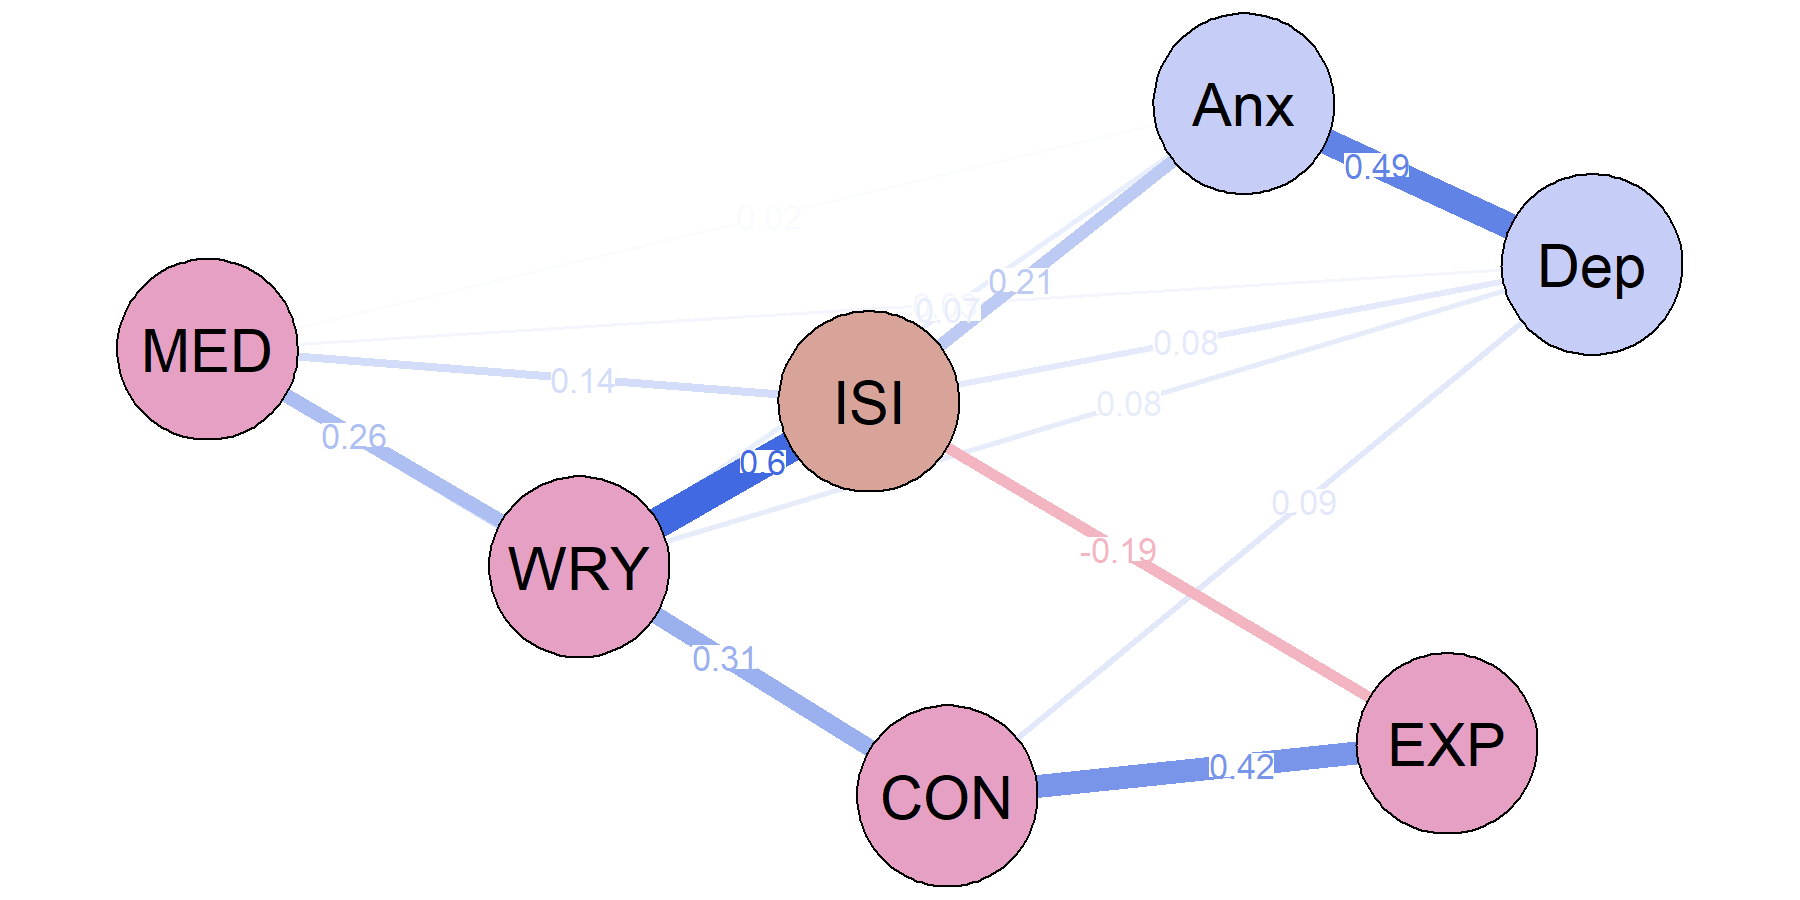
\includegraphics{img/network-conv-plot.png}

}

\caption{\label{fig-network-conv}Network of DBAS-16 factors, Insomnia
severity, Anxiety, and Depression. MED=Medication, WRY=Worry,
CON=Consequences, EXP=Expectations, ISI=Insomnia severity index,
Dep=Depression, Anx=Anxiety}

\end{figure}

\hypertarget{network-psychometrics-1}{%
\subsection{Network Psychometrics}\label{network-psychometrics-1}}

\hypertarget{derivation-of-the-factor-structure-in-the-training-sample}{%
\subsubsection{Derivation of the factor structure in the training
sample}\label{derivation-of-the-factor-structure-in-the-training-sample}}

First, we investigated potential redundancies between item pairs using
UVA. Based on weighted topological overlap (wTO) we found redundancies
between items 1 (\emph{Need 8 hours of sleep}) and 2 (\emph{Need to
catch up on sleep loss}) (wTO = 0.257), 3 (\emph{Consequences of
insomnia on health}) and 4 (\emph{Worried about losing control of
sleep}) (wTO = 0.318) and between items 6 (\emph{Better taking sleeping
pills}) and 15 (\emph{Medication as a solution}) (wTO = 0.308).

Before dealing with redundant items, we estimated the full DBAS-16's
dimensionality using EGA. To do this, we utilized GLASSO and TMFG
methods, with the Walktrap algorithm and Spearman correlation matrix,
due to our data's violation of multivariate normality. GLASSO produced
three dimensions, with a TEFI.vn index of -10.55, and TMFG produced
three with a TEFI.vn index of -11.02. We then assessed structural
consistency using the \texttt{bootEGA} function of \emph{EGAnet} with
parametric bootstrapping and 1000 replicates. The GLASSO model's
two-dimensional structure was replicated with a 56.6\% frequency across
bootstrap samples. The TMFG solution returned three dimensions in 48.6\%
of the replicates.

We then repeated these steps, considering redundancies identified prior
to the EGA. We first dealt with the redundancy between items 6 and 15,
keeping item 6 based on quantitative criteria and better generalization.
Item 15 had a larger maximum wTO to all other items (.112 vs.~.083),
lower item-total correlation corrected for item overlap and scale
reliability, and lower variance. The GLASSO model suggested three
dimensions with a TEFI.vn index of -11.54, while TMFG also suggested
three dimensions with a lower TEFI.vn of -9.78. Dimensionality
replication was still unsatisfactory for both models (TMFG: 48.6\%;
GLASSO: 50.8\%). We then dropped item 3 due to its higher maximum wTO,
lower item-total correlation, and variance. GLASSO produced three
dimensions again, and TMFG produced two dimensions. Dimensionality
replication slightly improved (TMFG: 69.8\%; GLASSO: 64.1\%), but
structural consistency for one dimension remained low in both models
(see Table dim-stab-table, NULL). Lastly, we maintained item 2 over item
1 due to its lower maximum wTO to all other items (respectively, .117
and .124) and higher variance. Both TMFG and GLASSO produced two
communities with identical item assignments.
Figure~\ref{fig-glasso-plots} and Figure~\ref{fig-tmfg-plots} show the
network plots obtained in each step of the analyses with the derivation
sample. The resulting network with two communities, without nodes 1, 3,
and 15, had the lowest TEFI.vn (-7.73) and higher replication rates
(TMFG: 87.1\%; GLASSO: 73.8\%), more satisfying structural consistency,
and better item stability into empirical dimensions, as shown in Table
@ref(tab:dim-stab-table). With no further redundancies to address, we
evaluated these results with the confirmation sample.

\begin{figure}

{\centering 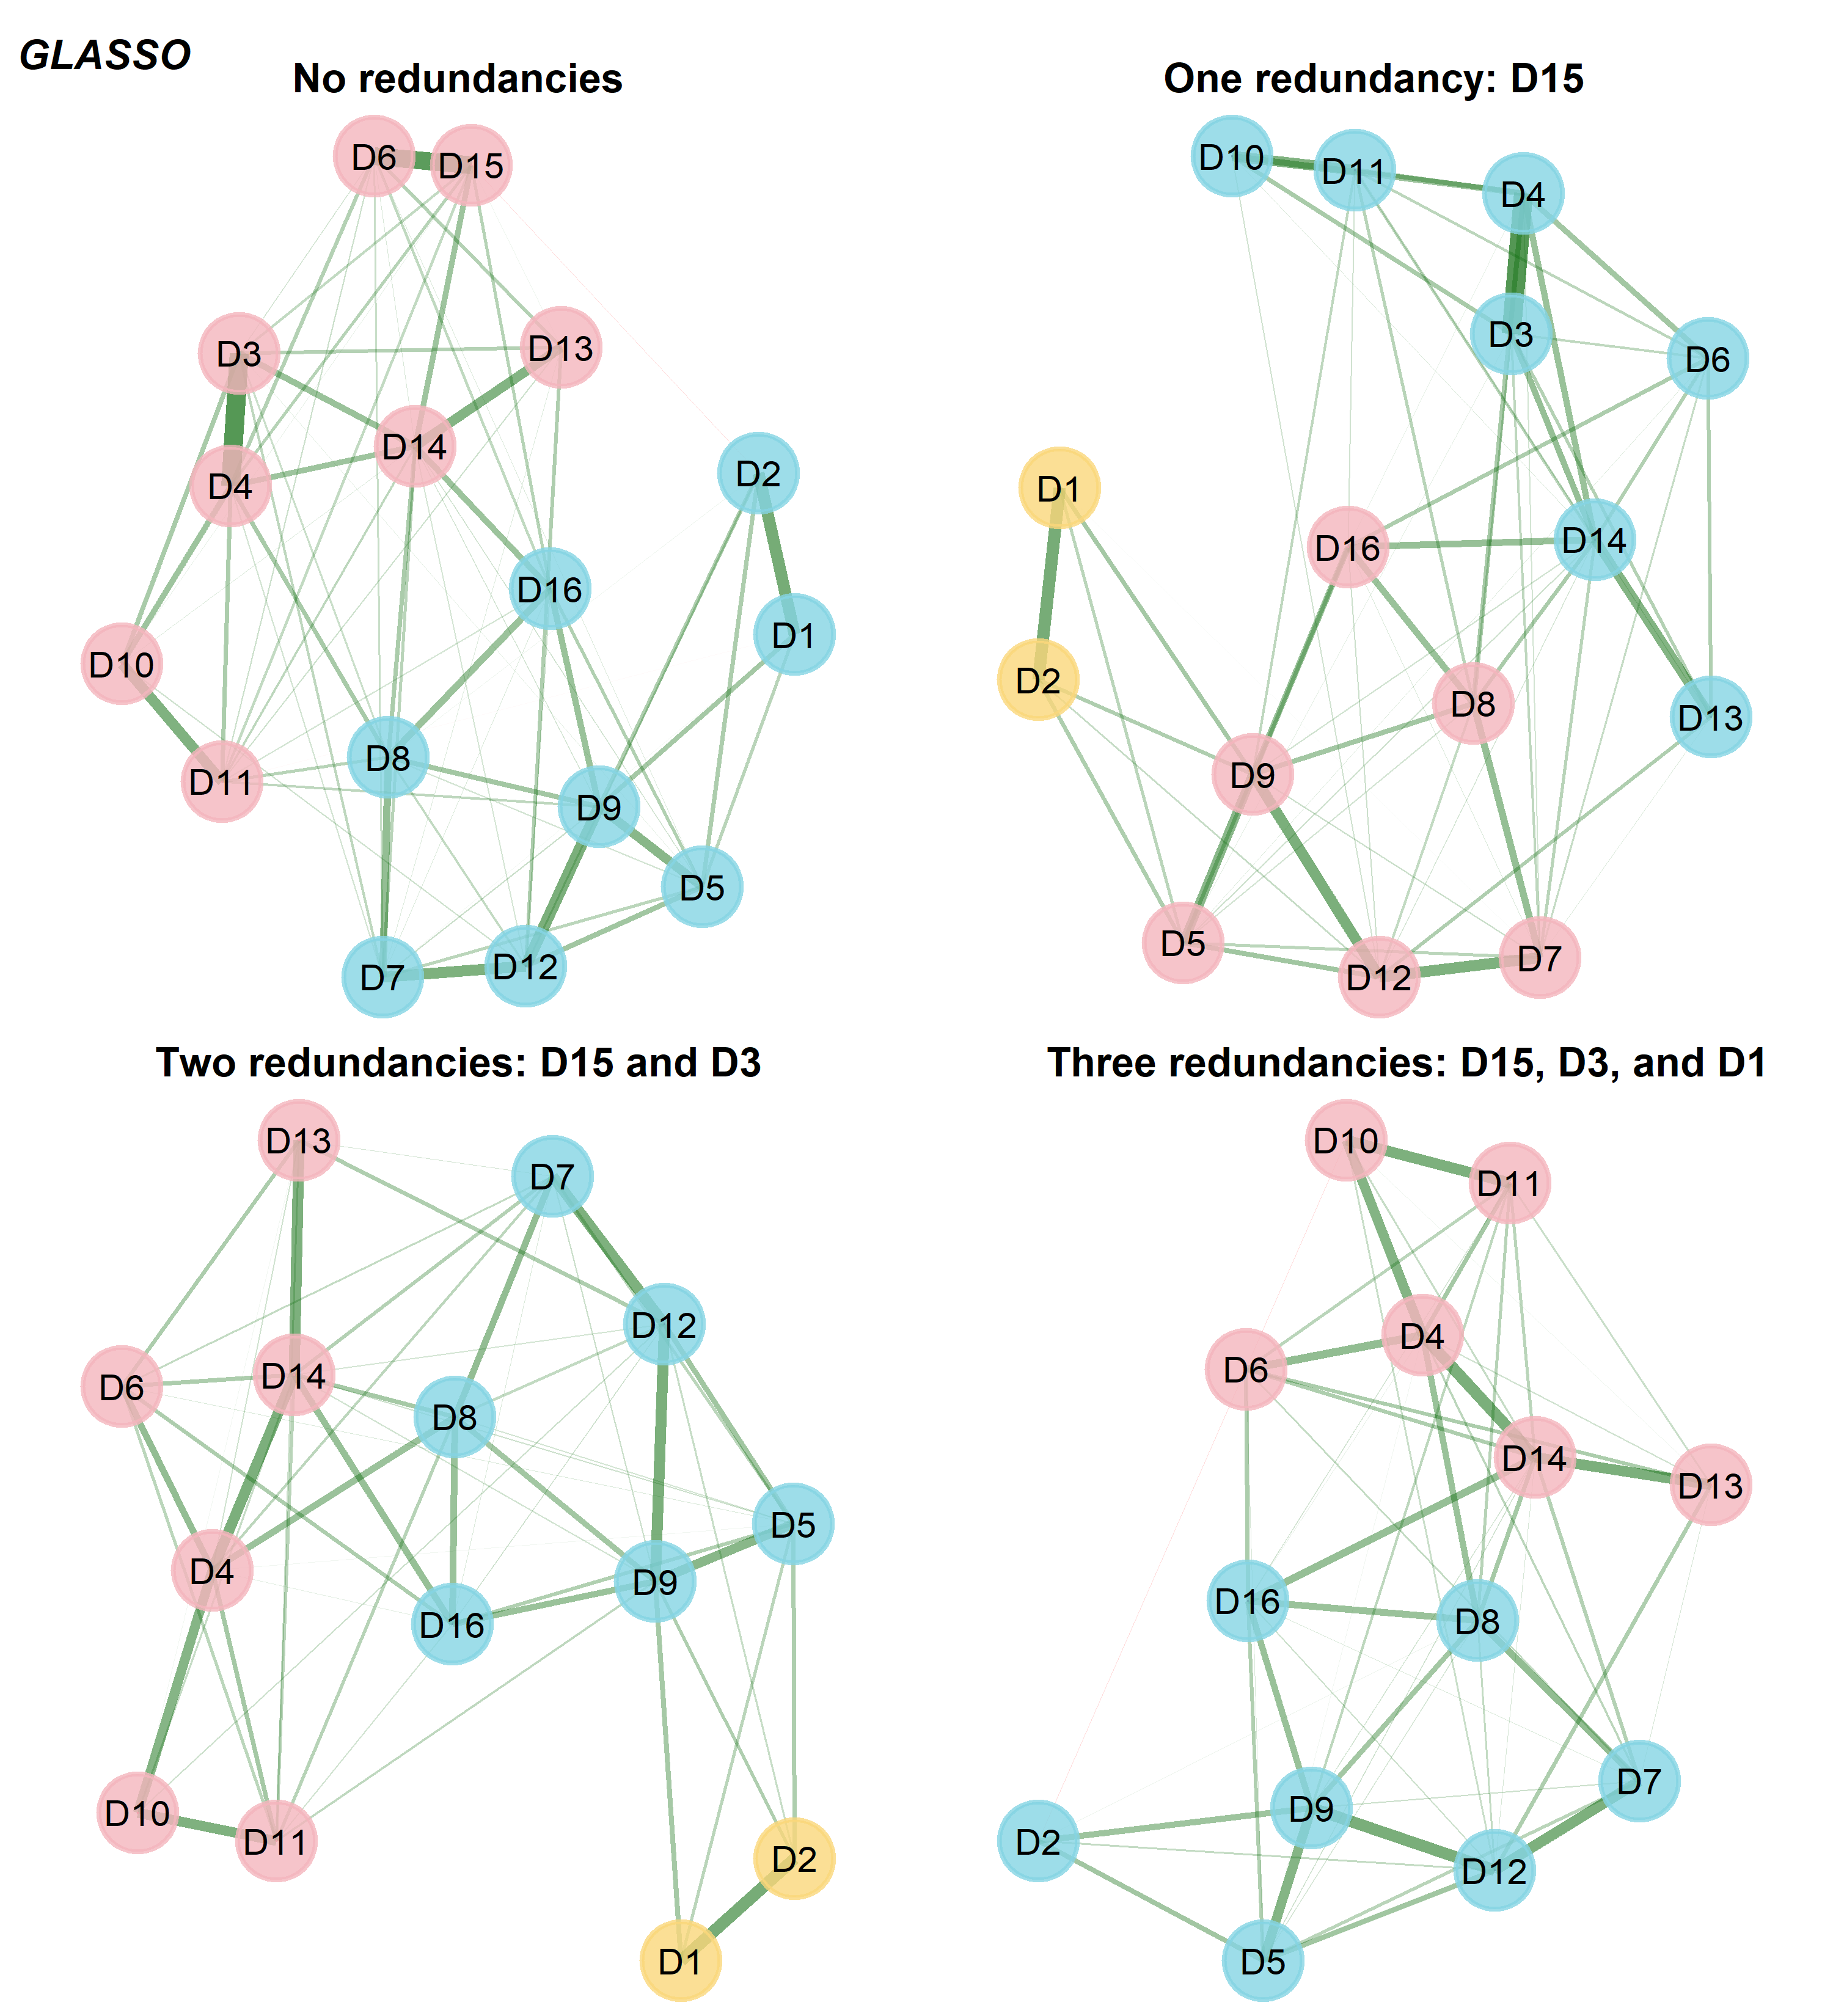
\includegraphics{img/glasso-plots-1.png}

}

\caption{\label{fig-glasso-plots}EGA GLASSO network plots for the
derivation sample.}

\end{figure}

\begin{figure}

{\centering 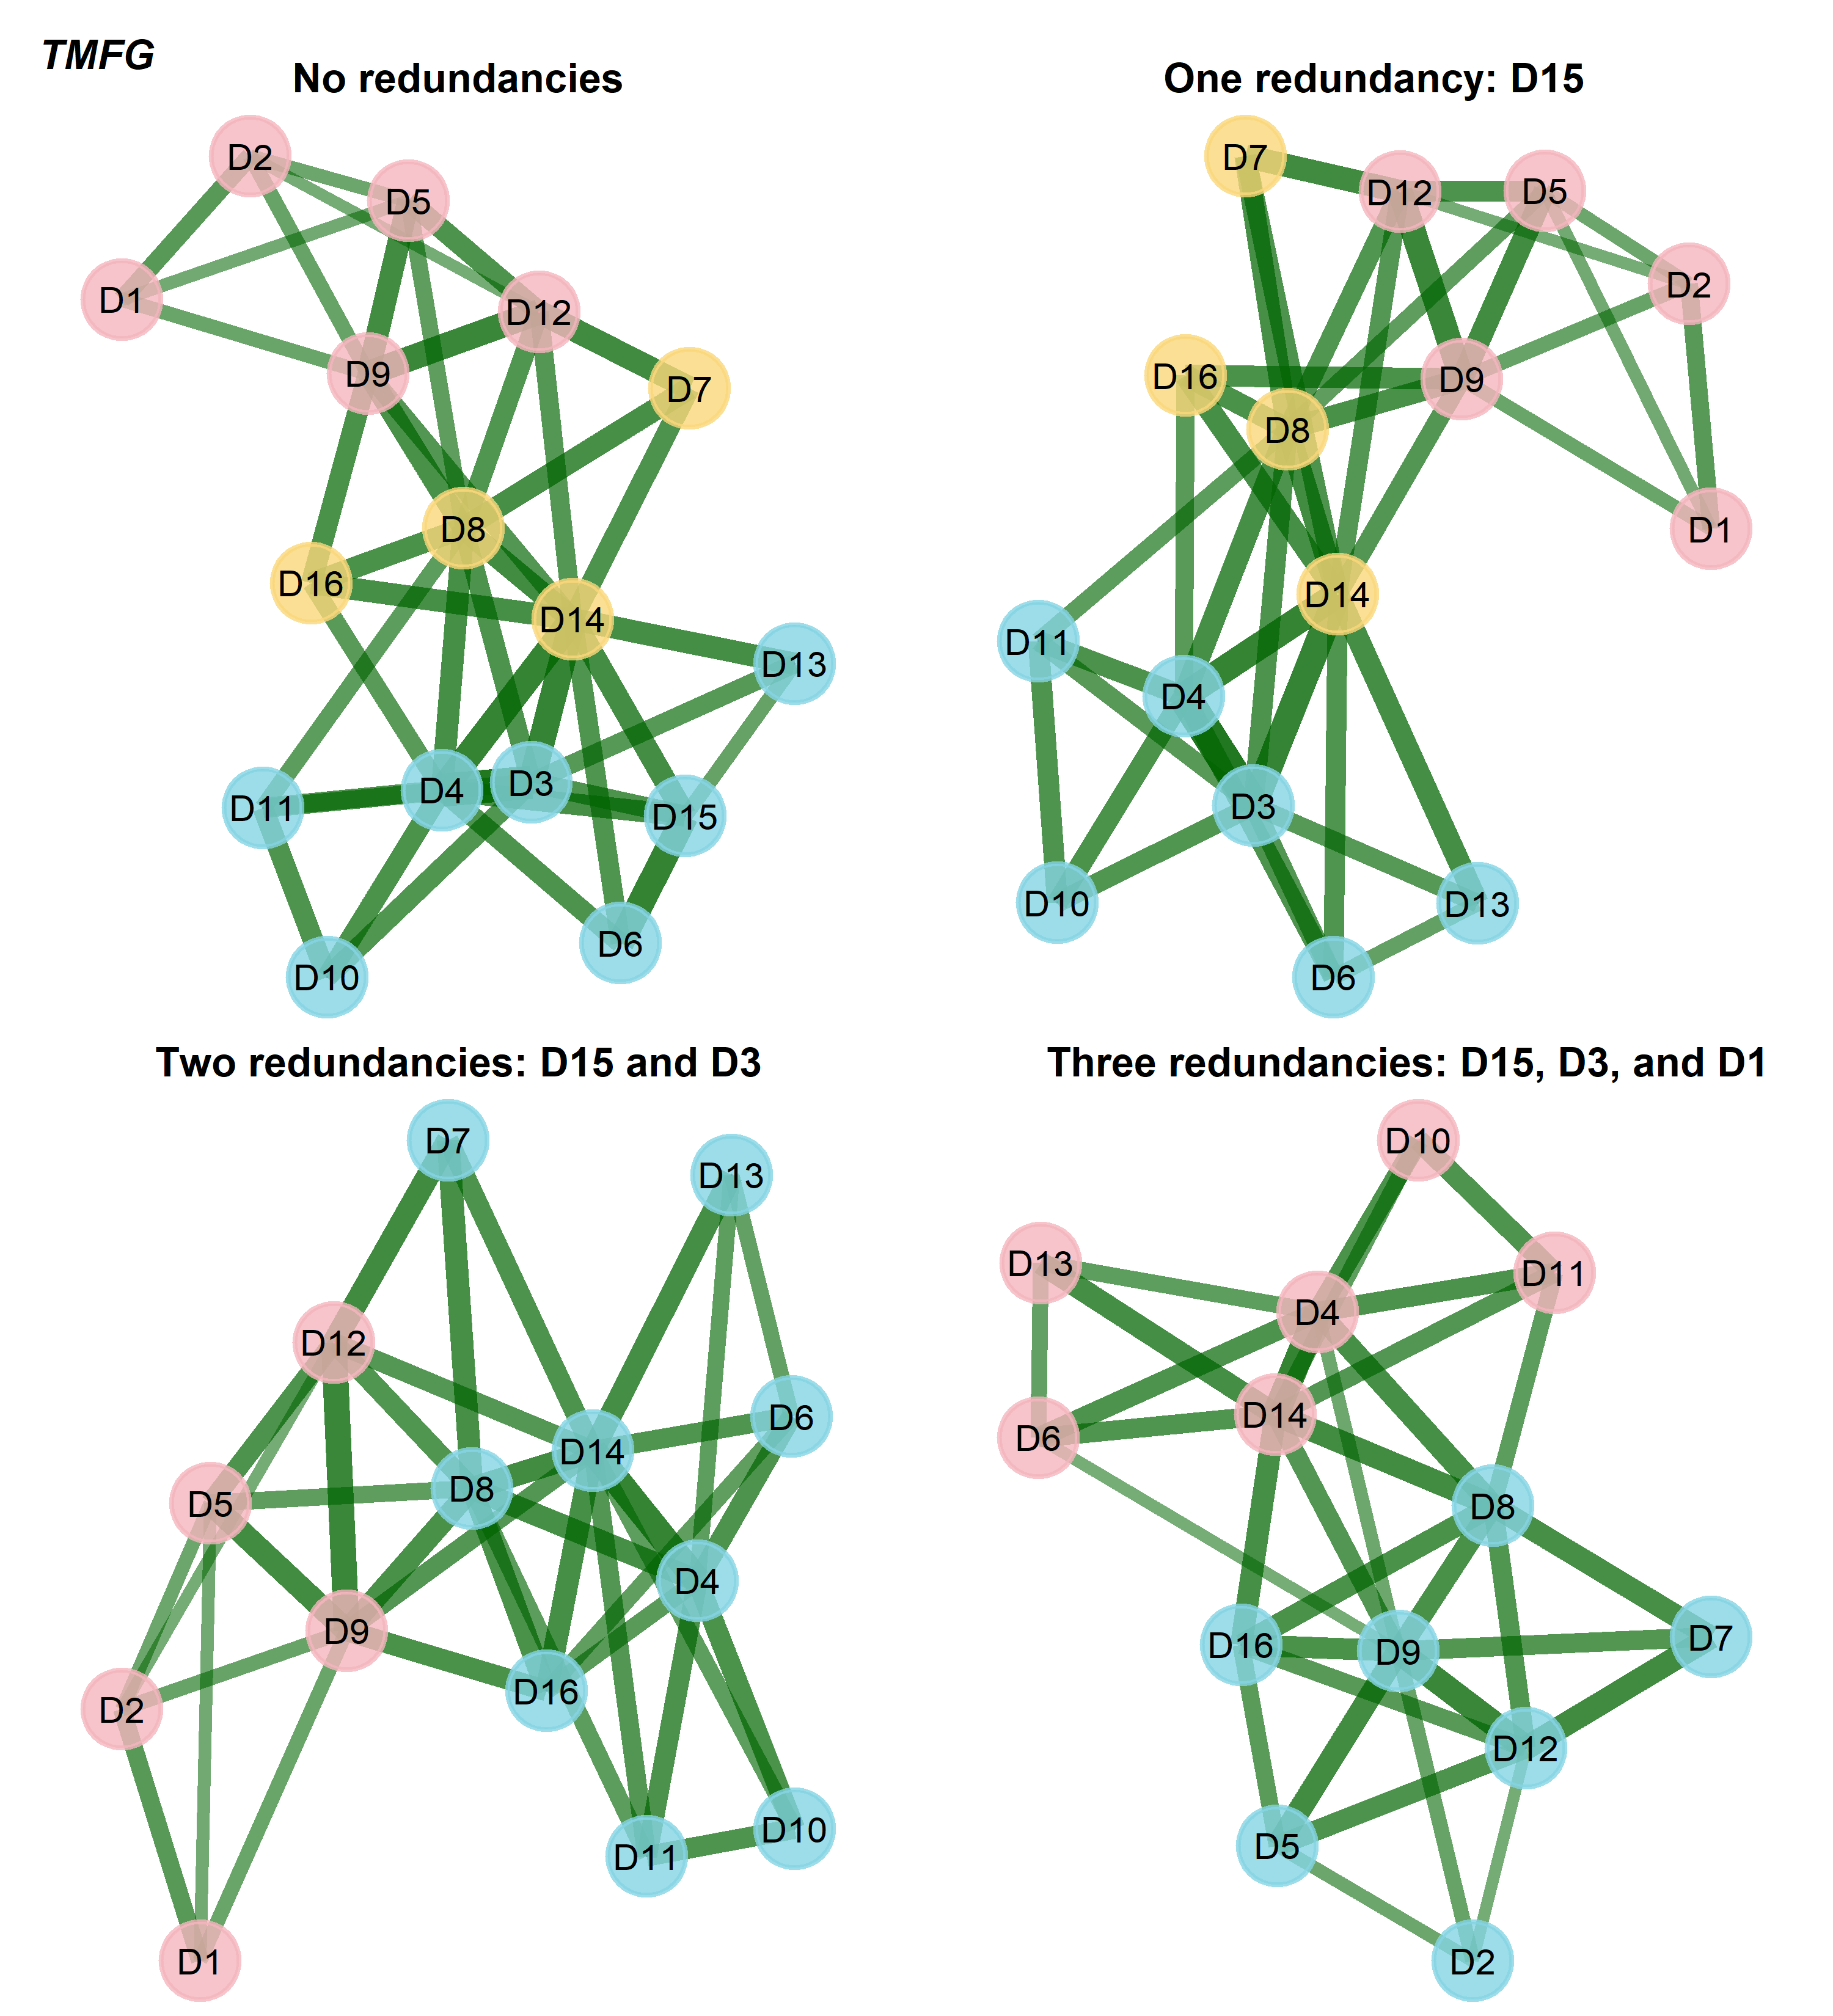
\includegraphics{img/tmfg-plots-1.png}

}

\caption{\label{fig-tmfg-plots}TMFG GLASSO network plots for the
derivation sample.}

\end{figure}

\hypertarget{confirmation-of-the-factor-structure-in-the-test-sample}{%
\subsubsection{Confirmation of the factor structure in the test
sample}\label{confirmation-of-the-factor-structure-in-the-test-sample}}

To determine if our results from the derivation sample were consistent,
we repeated the same procedures with the second half of our split
sample. UVA identified the same three redundancy pairs. We then ran the
EGA with GLASSO and TMFG, dropping items 1, 3, and 15 simultaneously.
Both methods returned two dimensions and replicated the item assignment.
Compared to GLASSO, TMFG had similar dimensionality replication rates
(TMFG: 92.5\%; GLASSO: 91.2\%) but significantly lower structural
consistency (Dimension 1: 64.6\% vs.~84.3\%; Dimension 2: 84.8\%
vs.~96\%). Overall, these results support the accuracy of the structure
obtained with GLASSO with the derivation sample.

Modeling the GLASSO model structure in a confirmatory factor analysis
yielded fit indices worse than a Level-3 misspecification obtained
through DFI (SRMR = .051, RMSEA = .093, CFI = .938): \(\chi^2\) (64, N =
693) = 302.592, RMSEA = .089 90\% CI {[}.079, .099{]}, CFI = .919, SRMR
= .063. Despite this, the GLASSO structure provided a better fit to our
data than the theory model with four factors: \(\Delta\chi^2\) (34) =
279.67, \emph{p} \textless{} .001, \(\Delta\)AIC = -9802.82,
\(\Delta\)BIC = -9852.77, \(\Delta\)RMSEA = .006, \(\Delta\)CFI = -.022,
\(\Delta\)SRMR = .012. Additionally, both dimensions had satisfactory
levels of internal consistency (\(\omega_{h1}\) = .84, \(\omega_{h2}\) =
.85).

Finally, we analyzed the full sample to test for invariance across
groups of good and bad sleepers in the EGA framework. First, we used
GLASSO to confirm the two-dimensional structure and item assignments
obtained from the derivation and confirmation sample. This structure was
successfully replicated in 93.1\% of 1000 bootstrap samples
(Median{[}SE{]} = 2{[}.26{]}). We also found excellent dimension
stability for Dimension 1 (90.5\%) and Dimension 2 (99.6\%), with item
stability ranging from .914 to 1.000.

Next, we examined whether the same nodes would form the same communities
for both groups (i.e., configural invariance). However, our initial
results indicated non-equivalent community structures for good and bad
sleepers, despite both samples conforming to a three-dimensional
structure, as shown in \textcite{fs-plots}. These results were somewhat
inconsistent when we ran the bootEGA, with the median number of
dimensions generated being 2 (SE\(_{gs}\) = .64, SE\(_{bs}\) = .61),
recovered across 67.8\% of the bootstrap samples for good sleepers'
sample and 53\% for bad sleepers' sample. Additionally, at least one
community of both typical structures had consistency levels below the
acceptable cutoff of .75, with some items having poor stability.

While configural invariance was not met, we investigated metric
invariance as if it was the case. Considering the two-dimensional
structure of the full sample, we found that only item 10 (``Sleep is
unpredictable'') had a statistically significant different network
loading performance after controlling the false discovery rate with the
Benjamini-Hochberg procedure.

\begin{figure}

{\centering 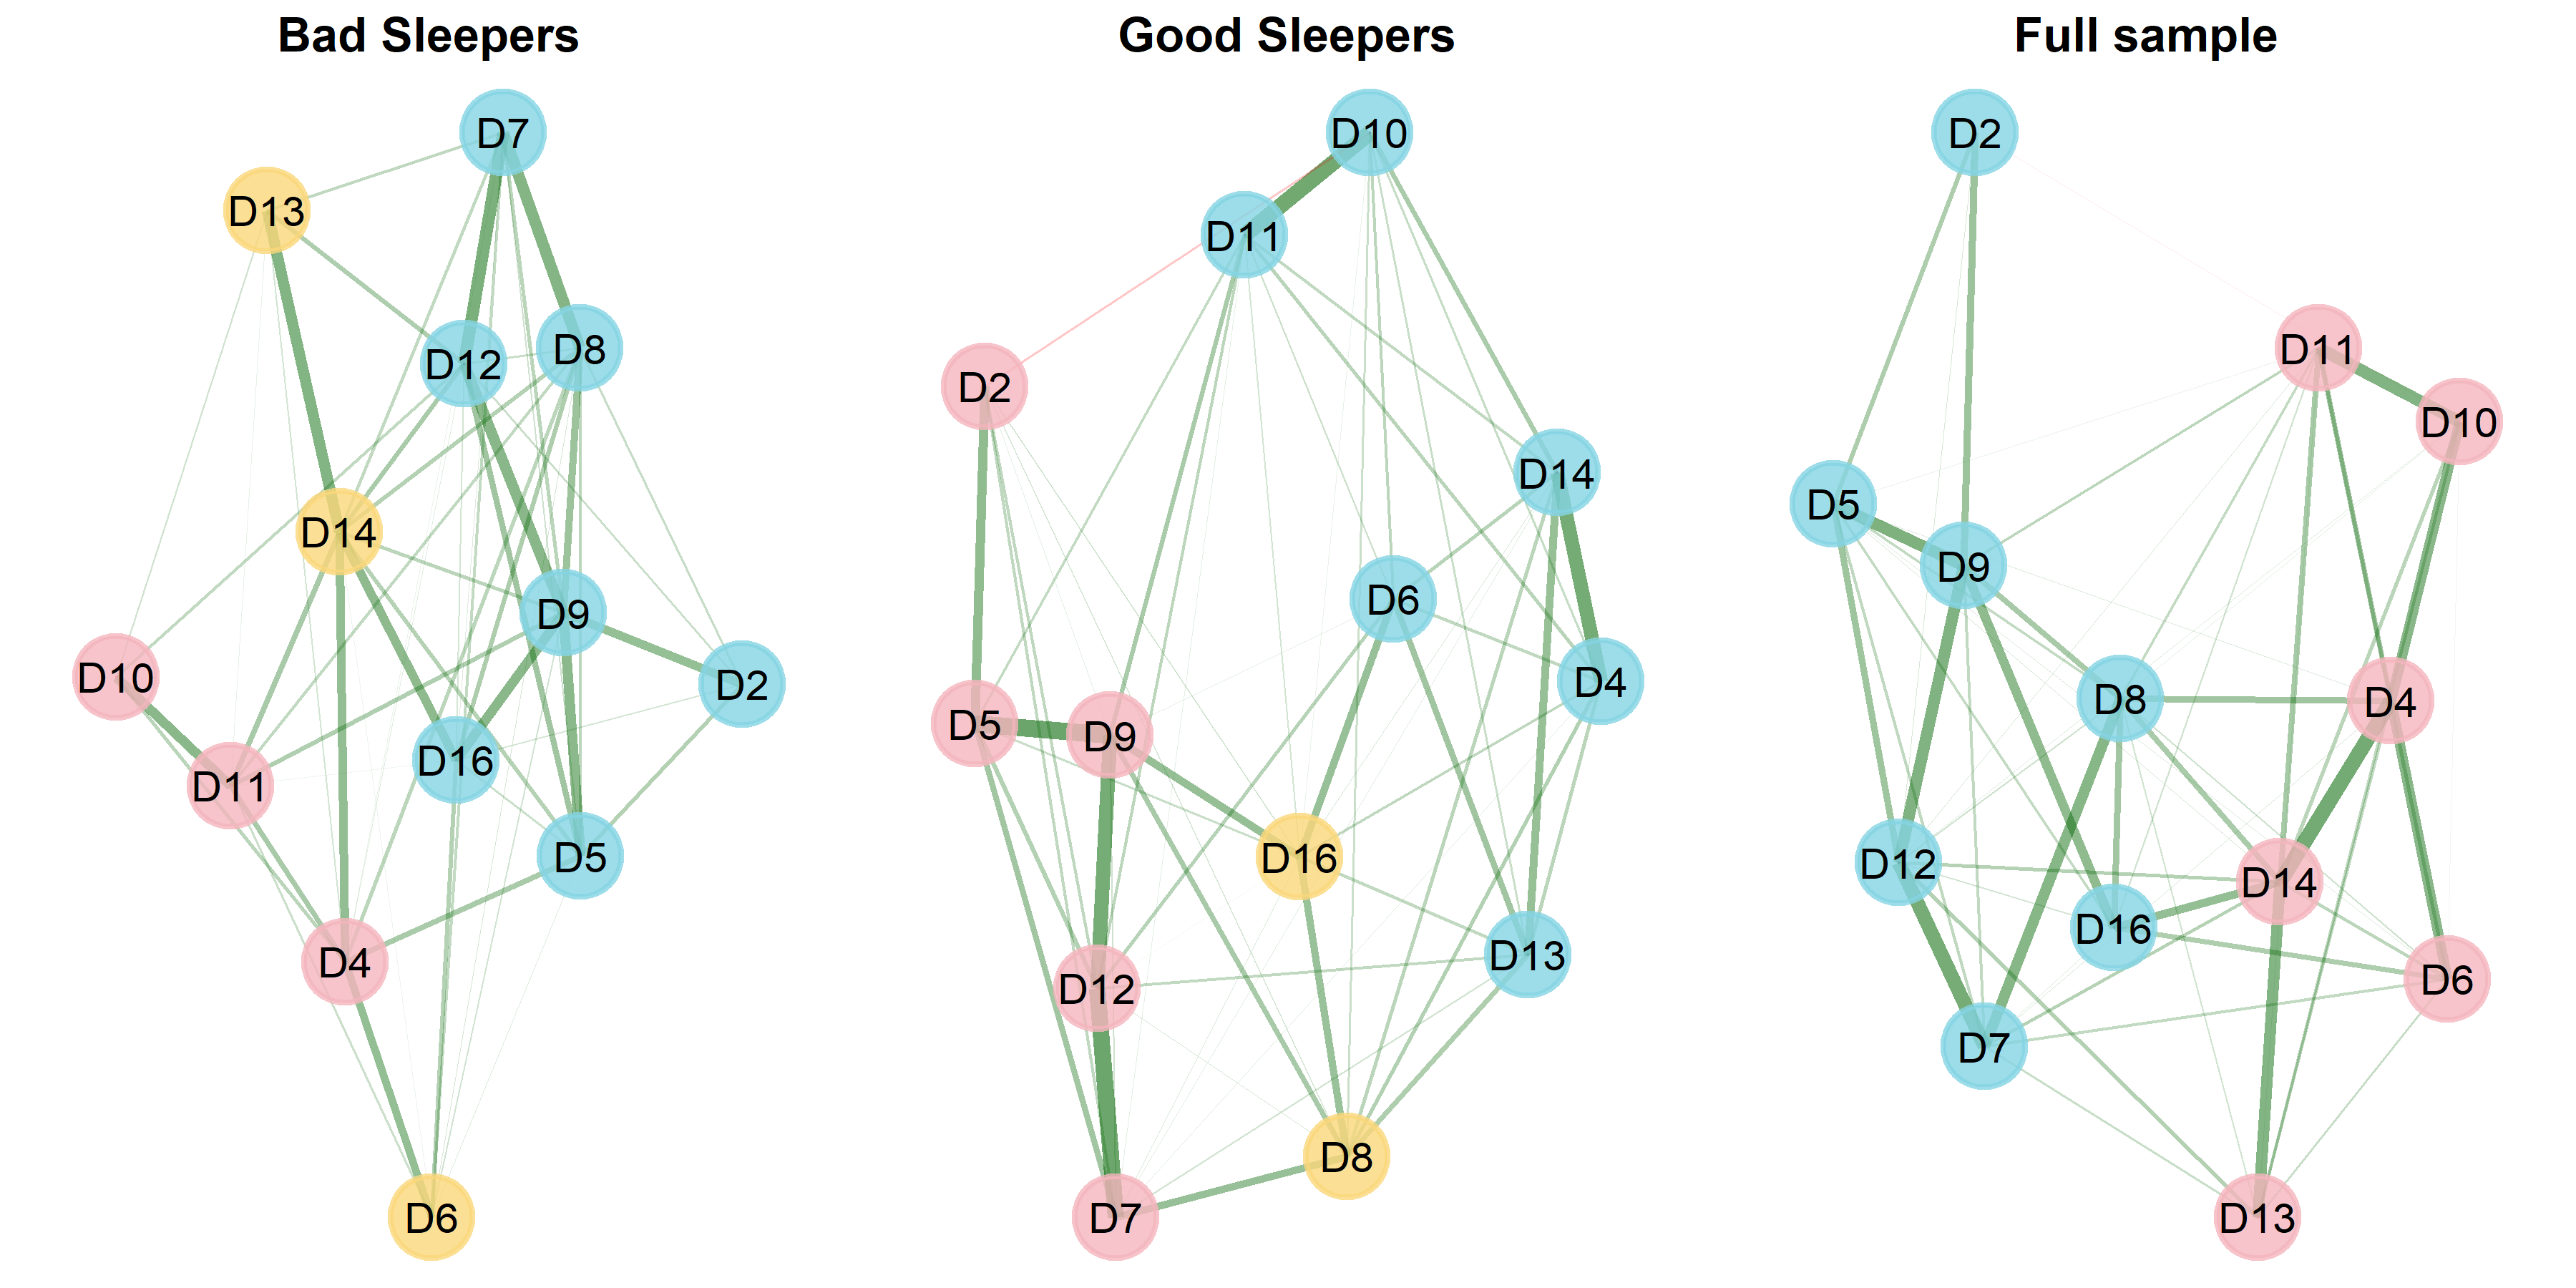
\includegraphics{img/fs-plots-1.png}

}

\caption{\label{fig-fs-plots}EGA GLASSO network plots for the full
sample.}

\end{figure}

\begin{table}[!h]

\caption{Stability of the EGA dimensionality 
      estimates across bootstrap samples}
\centering
\begin{tabu} to \linewidth {>{\raggedright}X>{\centering}X>{\centering}X>{\centering}X}
\toprule
\multicolumn{1}{c}{ } & \multicolumn{3}{c}{Dimensions } \\
\cmidrule(l{3pt}r{3pt}){2-4}
Model & 1 & 2 & 3\\
\midrule
\addlinespace[0.3em]
\multicolumn{4}{l}{\textit{Derivation sample (n = 693)}}\\
\addlinespace[0.3em]
\multicolumn{4}{l}{\textbf{No redundancies}}\\
\hspace{1em}\hspace{1em}TMFG & .832 & .939 & .226\\
\hspace{1em}\hspace{1em}GLASSO & .543 & .785 & .\\
\addlinespace[0.3em]
\multicolumn{4}{l}{\textbf{One redundancy (15)}}\\
\hspace{1em}\hspace{1em}TMFG & .888 & .909 & .240\\
\hspace{1em}\hspace{1em}GLASSO & .910 & .755 & .546\\
\addlinespace[0.3em]
\multicolumn{4}{l}{\textbf{Two redundancies (15, 3)}}\\
\hspace{1em}\hspace{1em}TMFG & .168 & .844 & .\\
\hspace{1em}\hspace{1em}GLASSO & .588 & .949 & .693\\
\addlinespace[0.3em]
\multicolumn{4}{l}{\textbf{Three redundancies (15, 3, 1)}}\\
\hspace{1em}\hspace{1em}TMFG & .342 & .810 & .\\
\hspace{1em}\hspace{1em}GLASSO & .661 & .863 & .\\
\addlinespace[0.3em]
\multicolumn{4}{l}{\textit{Confirmation sample (n = 692)}}\\
\addlinespace[0.3em]
\multicolumn{4}{l}{\textbf{Three redundancies (15, 3, 1)}}\\
\hspace{1em}\hspace{1em}TMFG & .646 & .848 & .\\
\hspace{1em}\hspace{1em}GLASSO & .843 & .960 & .\\
\addlinespace[0.3em]
\multicolumn{4}{l}{\textit{Full sample (n = 1385)}}\\
\addlinespace[0.3em]
\multicolumn{4}{l}{\textbf{Three redundancies (15, 3, 1)}}\\
\hspace{1em}\hspace{1em}GLASSO & .905 & .996 & .\\
\bottomrule
\end{tabu}
\end{table}

\hypertarget{discussion}{%
\section{DISCUSSION}\label{discussion}}

Dysfunctional beliefs and attitudes about sleep feature in many popular
models of insomnia and are investigated widely using the DBAS-16
\autocite{tang2023}. With this study, we produced a Brazilian-Portuguese
version of the questionnaire. We demonstrated its semantic and
psychometric equivalence to the original version, making its use
suitable for the Brazilian population. Additionally, this study was the
first to show that the DBAS-16's structure was noninvariant across good
and bad sleepers and to attest temporal stability using the measurement
invariance framework. Despite acceptable model fit indices in the
confirmatory analysis, they were only obtained by correlating residuals.
On top of that, modification indices also suggested that the model could
be improved with the addition of cross-loadings. Using network
psychometrics, we found that (1) items 1, 3, and 15 could be deleted
without losing information, (2) two dimensionalities better represent
the underlying structure of the DBAS scores, and (3) the item referring
to the belief that sleep is unpredictable was noninvariant across good
and bad sleepers.

Our analysis of DBAS-16's structure confirms much of previous research
\autocite{morin2007a,castillo2023,boysan2010}. The four-factor structure
had acceptable indices by traditional and dynamic fit indices. The
``worry about sleep'' and ``consequences'' subscales had strong internal
consistency, while the ``expectations'' and ``medication'' subscales had
modest values. These results suggest that the idea that these 16 items
assessing dysfunctional beliefs and attitudes about sleep conform to a
four-factor structure is questionable. Reliability of ``expectations''
and ``medication'' subscales could be affected by the scarce number of
items composing them and low factor loadings (ranging from .58 to .68).
Modifying a model based on modification indices can be risky as it might
not generalize to other samples \autocite{maccallum1992}, but items 3
and 4 have been found to have correlated residual variance in previous
research \autocite{morin2007a,boysan2010,castillo2023}. We can at least
infer that these items share something in common that is not accounted
for by the latent factor, such as similar wording or content overlap.
Our results are congruent with past confirmatory analyses of DBAS-16's
four-factor structure and contribute as the first analysis with a large
(\textgreater1000) clinical sample.

Our study found that model structure and factor loadings remained
consistent over 14 days. However, we did not find conclusive evidence of
item intercept equivalence during this period. There were no significant
differences in model fit between good and bad sleepers. Nevertheless,
the items' loadings on the factors varied across groups. These findings
have critical implications for studies assessing dysfunctional beliefs
before and after an intervention. Although the DBAS-16 remained stable
over time, participants did not change in insomnia severity status.
Improvement in insomnia symptoms can likely change how DBAS-16 items are
interpreted. Hence, researchers should not take measurement invariance
for granted but test it because a possible decrease in dysfunctional
beliefs about sleep cannot be interpreted straightforwardly.

Regarding convergent validity, except for ``expectations,'' DBAS-16
factors had positive moderate-to-strong correlations with insomnia
severity, anxiety and depression. These findings are not unexpected, as
\textcite{morin2007a} observed a similar pattern but retained the
``expectations'' items for their clinical relevance. A statistical
network revealed the centrality of the ``worry'' node and the negative
partial correlation between sleep expectations and insomnia severity.
The first development highlights the ``worry about sleep'' importance in
the flow of information through the network. It also agrees with
\textcite{clemente2023} IRT analysis showing that the ``worry about
sleep'' subscale provided the most information and the highest level of
precision. \textcite{clemente2023} found that items measuring
expectations provided more information about individuals with lower
unhelpful beliefs about sleep. Their results help us understand the
negative partial correlation between expectations about sleep and
insomnia severity since these beliefs might also be common to good
sleepers and are not good indicators of sleep problems. Our results also
answer their call to evaluate their findings with a clinical sample.

The second objective of this research was to explore the structure of
DBAS-16. UVA identified three pairs of items that were locally dependent
with a wTO score greater than .25. These pairs were item 1 (``Need 8
hours of sleep'') and item 2 (``Need to catch up on sleep loss''), item
3 (``Consequences of insomnia on health'') and item 4 (``Worried about
losing control of sleep''), and item 6 (``Better taking sleeping
pills'') and item 15 (``Medication as a solution''). We removed items 1,
3, and 15 based on quantitative and qualitative criteria. Some may
question why we considered items 1 and 2 redundant, as their wTO score
slightly exceeded the cutoff and originally formed a latent factor. We
believe that the emergence of a minor factor comprising only these two
items was caused by not considering local dependence. Our decision to
drop item 15 disagrees with \textcite{clemente2023} option for keeping
it due to the highest discriminatory value among the items in the
``medication'' subscale and deleting item 6 due to its flat item
characteristic curve. This example illustrates that our study is not
advocating for a shorter ``DBAS-13'' as there may be more aspects to
consider when deciding on a specific item removal criterion.
Nonetheless, we achieved a two-dimensional structure with excellent item
and structure stability levels by removing those items.

Our research using EGA revealed that two dimensions accurately reflect
our sample's underlying structure of dysfunctional beliefs and attitudes
toward sleep. Dimension 1 is composed of nodes from the original
``consequences of insomnia'' factor (items 5, 7, 9, 12, and 16), along
with item 2 (``When I don't get a proper amount of sleep on a given
night, I need to catch up on the next day by napping or sleeping
longer'') from ``medication,'' and item 8 (``When I sleep poorly on one
night, I know it will disturb my sleep schedule for the whole week'')
from ``worry about sleep.'' Since items 2 and 8 share a semantic value
related to the consequences of poor sleep, we may keep the original
terminology and label Dimension 1 as ``Consequences of insomnia.''
Dimension 2 is composed of the remaining items from the ``worry about
sleep'' subscale (items 4, 10, 11, and 14) and item 6 (``In order to be
alert and function well during the day, I believe I would be better off
taking a sleeping pill rather than having a poor night's sleep'') and 13
(``I believe insomnia is essentially the result of a chemical
imbalance'') from ``medication.'' Assuming that worry about sleep leads
to medication use, we can label Dimension 2 as ``Worry about sleep.''

Using a new technique in the EGA framework to test measurement
invariance, we discovered that the network structure was noninvariant
for both good and bad sleepers, just like the theory model. However, we
couldn't determine the best structure for either group due to low
structure stability. We found that item 10 (``I can't ever predict
whether I'll have a good or poor night's sleep'') was the only
noninvariant regarding network loadings. This result supports Clemente
et al.'s \autocite*{clemente2023} discovery that item 10 effectively
distinguishes between good and bad sleepers. Regardless, we must be
cautious when interpreting this finding since we cannot assume that the
network structure is identical for both groups.

\hypertarget{limitations}{%
\subsection{Limitations}\label{limitations}}

Our research was the first to explore the potential insights that
network psychometrics can provide on the DBAS-16. However, it is
important to acknowledge certain limitations in our findings. The EGA
methods we used were selected based on simulation studies, which may not
entirely reflect the nature of our data. EGA is a relatively new
technique, so further research is needed to address unanswered questions
\autocite{golino2022}. For example, our preliminary analysis showed that
TMFG and GLASSO produced different structures. Additionally, selecting
Louvain over Leading Eigenvalue to test for unidimensionality could lead
to the assumption of a unidimensional structure for poor sleepers. While
we based our choices on the best available evidence, these results are
preliminary and suggest a direction for further investigation.

In both our confirmatory and exploratory analyses, we found that certain
biases could have influenced our data. First, the participants who had
sleep problems were seeking treatment for insomnia, which meant that
they were likely to be more severely affected by the disorder.
Additionally, our data was unbalanced towards bad sleepers, which could
have also contributed to our heavily skewed data and low statistical
power to test measurement invariance across groups. Secondly, we
administered the questionnaires online, and participants could not leave
blank fields. This may have introduced bias, as participants may have
provided an answer even if it did not apply to their situation. Third,
we did not include elderly people; therefore, the outcomes cannot be
generalized to all adults with insomnia. Fourth, most of our sample
comprised white women with a university degree. Future studies should
focus on collecting more representative samples, including those with
lower educational levels. Fifth, it is important to note that our study
used the Brazilian-Portuguese adaptation of the DBAS-16. Although we
ensured that it was equivalent to the English version, specific terms or
cultural characteristics may have influenced the results. These findings
should be replicated in samples from different countries. Finally, we
used the same total sample for derivation and confirmation. We tried to
mitigate this issue by splitting the sample into two halves, but we
recognize that it cannot eliminate sampling bias. Therefore, it is
highly recommended that our findings be replicated using a larger, more
diverse, and older sample, ensuring a greater balance between good and
poor sleepers. Additionally, further research should test longitudinal
invariance over at least eight weeks to reflect typical
cognitive-behavioral treatment protocols for insomnia
\autocite{harvey2014}.

\hypertarget{conclusion}{%
\section{CONCLUSION}\label{conclusion}}

Our research shows that the DBAS-16 is suitable for a
Brazilian-Portuguese-speaking population. It also provides initial
insights into the network structure of dysfunctional beliefs and
attitudes about sleep. Our findings support a two-factor structure, as
\textcite{clemente2023} suggested. We achieved greater stability in the
structure by removing locally dependent items. Although our results
require further confirmation and refinement, they can assist clinicians
and researchers in gaining a better understanding of how dysfunctional
beliefs and attitudes about sleep are organized. This can provide
valuable insights into beliefs that may be more or less significant in
understanding this concept.


\printbibliography[title=REFERÊNCIAS]


\end{document}
